% \documentclass{apnet18}
\documentclass[sigconf,10pt]{acmart}

% \usepackage{times}
% \usepackage{epsfig}
% \usepackage[TABBOTCAP]{subfigure}
% \usepackage{tabularx}
% \usepackage{graphicx}
\usepackage{color}
\usepackage{xspace}
% \usepackage{thumbpdf}
% \usepackage{listings}
% \usepackage{verbatim}
% \usepackage{hyperref}
% \usepackage{booktabs}
\usepackage{colortbl}

% \usepackage{colortbl,booktabs}%
\usepackage{subfigure}
\usepackage{amsmath}
\usepackage{algorithm}    
\usepackage{algorithmic} 

\geometry{left=0.75in,right=0.75in,top=0.875in,bottom=0.875in}

% \usepackage{fancyhdr} 
% \renewcommand{\headrulewidth}{0pt} 
% \renewcommand{\footrulewidth}{0pt}

% \maketitle 
% \thispagestyle{fancy} 
% \fancyhead{} 
% \lhead{} 
% \lfoot{978-1-5386-4362-4/18/$31.00 \copyright 2018 IEEE} 
% \cfoot{} 
% \rfoot{}





% \hypersetup{pdfstartview=FitH,pdfpagelayout=SinglePage}

% \setlength\paperheight {11in}
% \setlength\paperwidth {8.5in}
% \setlength{\textwidth}{7in}
% \setlength{\textheight}{9.25in}
% \setlength{\oddsidemargin}{-.25in}
% \setlength{\evensidemargin}{-.25in}

%\setlength{\headsep}{0in}
%\pagenumbering{arabic}


\renewcommand\thesection{\arabic{section}} 

\newcommand{\eg}{{\it e.g.,}\xspace}
\newcommand{\ie}{{\it i.e.,}\xspace}
\newcommand{\fillme}{{\bf XXX}~}
\newcommand{\jc}[1]{{\footnotesize\color{blue}{[JC: #1]}}} %[JC: #1]}}}
\newenvironment{packeditemize}{\begin{list}{$\bullet$}{\setlength{\itemsep}{0.5pt}\addtolength{\labelwidth}{-4pt}\setlength{\leftmargin}{\labelwidth}\setlength{\listparindent}{\parindent}\setlength{\parsep}{1pt}\setlength{\topsep}{0pt}}}{\end{list}}

% \newcommand{\tightcaption}[1]{\vspace{-0.4cm}\caption{{\textit{\textbf{#1}}}}\vspace{-0.38cm}}
\newcommand{\tightcaption}[1]{\vspace{-0.4cm}\caption{{\textit{\textbf{#1}}}}\vspace{-0.0cm}}

\newcommand{\tightsection}[1]{\vspace{-0.25cm}\section{#1}\vspace{-0.08cm}}
\newcommand{\tightsubsection}[1]{\vspace{-0.35cm}\subsection{#1}\vspace{-0.08cm}}
%\newcommand{\tightsection}[1]{\vspace{-0.0cm}\section{#1}\vspace{-0.0cm}}
%\newcommand{\tightsubsection}[1]{\vspace{-0.0cm}\subsection{#1}\vspace{-0.0cm}}
\newcommand{\tightsubsubsection}[1]{\vspace{-0.01in}\subsubsection{#1}\vspace{-0.01cm}}

\setlength{\textfloatsep}{2pt}

\begin{document}

	


%%%%%%%%%%%% THIS IS WHERE WE PUT IN THE TITLE AND AUTHORS %%%%%%%%%%%%

% \title{Dante: An FOV-Aware FEC-Based Protocol for 360-Degree Video Streaming}
\title{Dante: Enabling FOV-Aware Adaptive FEC Coding \\for 360-Degree Video Streaming}


\author{\large{
Zhetao Li$^{\dagger}$, Fei Gui$^{\dagger}$, Jinkun Geng$^{\circ}$, Dan Li$^{\circ}$, Zhibo Wang$^{\Diamond}$, Junfeng Li$^{\circ}$, Yang Cheng$^{\circ}$, Usama Zafar$^{\circ}$\\ \\
$^{\dagger}$Xiangtan University~~~~~~~~~~~~  $^{\circ}$Tsinghua University~~~~~~~~~~~~~  $^{\Diamond}$Wuhan University}}

% Zhe tao Li (Xiangtan University)
%               Fei Gui (Xiangtan University)
%               Jinkun Geng (Tsinghua University)
%               Dan Li* (Tsinghua University)
%               Zhibo Wang (Wuhan University)
%               Junfeng Li (Tsinghua University)
%               Yang Cheng (Tsinghua University)
%               Usama Zafar (Tsinghua University)


\copyrightyear{2018}
\acmYear{2018}
\setcopyright{acmcopyright}
\acmConference[APNet '18]{2nd Asia-Pacific Workshop on
	Networking}{August 2--3, 2018}{Beijing, China}
\acmBooktitle{APNet '18: 2nd Asia-Pacific Workshop on Networking, August
	2--3, 2018, Beijing, China}
\acmPrice{15.00}
\acmDOI{10.1145/3232565.3232569}
\acmISBN{978-1-4503-6395-2/18/08}

\renewcommand{\shortauthors}{ F. Gui et al.}

%\thispagestyle{empty}


	
%%%%%%%%%%%%%  ABSTRACT GOES HERE %%%%%%%%%%%%%%
\begin{abstract}
As 360-degree videos grow dramatically in popularity, more 
applications demand the ability to stream 360-degree videos to 
wirelessly connected devices, such as smartphone headsets. However, 
the limited capacity and the unstable network conditions make 
wireless networks ill-suited to the requirements of 
360-degree videos---high resolution and low delay. One common 
approach is to take advantage of the fact that the viewer only
watches a small portion of the video around the 
field of view (FOV). This allows for better allocation of 
network bandwidth by prioritizing content the viewer actually watches. 
Previous efforts on 360-degree videos have largely focused on 
adapting the encoded bitrate to optimize video quality in the 
time-varying FOV. This paper follows the general FOV-aware approach
but uses a different technique. Rather than adapting bitrate, 
we explore the opportunities of a custom underlying 
transport protocol for 360-degree videos.  In particular, we
make a case for using Forward Error Correction (FEC) 
coding over UDP to reduce video streaming delay (a key 
limitation of all TCP-based approaches).
We present {\em Dante}, an FOV-aware UDP-based video streaming protocol 
that adapts to changing network conditions by dynamically
choosing FEC redundancy levels based on how close the video content is
to the FOV region. Experimental 
results show that Dante improves video quality (PSNR) by 20\% to
30\% over traditional UDP-based video 
streaming protocols and 40\% over FOV-aware DASH.
\end{abstract}

\maketitle

%360-degree videos have been widely applied due to its unprecedented immersive experience. The appreciation of watching 360-degree videos
%on untethered mobile devices, such as smartphone headsets,
%is considered to be a more promising trend, which, however, is hampered by the
%poor Quality of Experience (QoE), subject to limited bandwidth and error-prone characteristic of wireless networks.
%Fortunately, the key observation that only a small portion of a 360-degree video is
%perceived by users at any time, i.e., Field Of View (FOV), implies that unequal attention
%should be given different regions spatially and can
%be utilized to mitigate dependence on stable network condition and ultra-high bandwidth. Currently, the state-of-the-art schemes, like FOV-aware tile-based streaming in the application layer, almost based on FOV-aware bit-rate adaptation, transport protocol of which, however, fails to consider FOV. So, we propose an application-layer protocol, reliability scheme of which is FOV-aware and performs hierarchical protection to boost QoE of 360-degree videos in mobile scenarios. Experiments demonstrate our protocol achieves desirable improvements over the reference schemes in QoE of 360-degree videos.

% \section{Introduction}

% 360 degree videos are important
360-degree videos are coming to age, which has been driven by content
providers (\eg CNN, New York Times) serving more immersive content (\eg 
NBC broadcasting the 2018 Winter Olympics in VR~\cite{NBC_olympic_360}), as well as 
by more application platforms~\cite{google_developers,facebook360} and 
devices (\eg Samsung smartphone headset~\cite{SUMSUNG_HEADSET}).
However, streaming 360-degree videos to mobile devices through wireless
networks remains a substantial challenge.

% why it's challenging
To provide true immersive experience, the 360-degree video must be streamed
in high resolution and within a small bounded delay.

\begin{packeditemize}
% low delay
\item {\em Stringent delay constraint:} 

To prevent simulator sickness \cite{Simulator_Sickness} and to provide good Quality of Experience (QoE), the vendors of HeadMounted Displays (HMD) recommend that the video systems
react to head movements as fast as the HMD refresh rate, i.e., frames per second (fps).
Since fps of state-of-the-art HMDs is 120 Hz,
the whole system should react in less than 10 ms. These stringent delay constraints render many traditional streaming 
protocols (\eg~\cite{MPEG-DASH},~\cite{FESTIVE}) insufficient.

%\jc{reword the last sentence. what's "application round-trip latency"? why "sickness" is caused by some "refresh rate"?} These stringent delay constraints render many traditional streaming  protocols (\eg~\cite{??,??}) insufficient.

% high bandwidth
\item {\em High-bandwidth consumption:}
Moreover, 360-degree videos require high bandwidth to stream videos in
high resolution, ideally, over the whole 360-degree sphere; \eg the 
bitrate of an 8K 360-degree video feed encoded at a frame rate of 60 fps
(frames per second) with HEVC~\cite{HEVC} is $\sim$100Mbps. According to
OpenSignal~\cite{opensignal}, almost a half of the 77 surveyed 
countries in 2017 over the world only have access to 4G cellular 
networks of 10-25 Mbps.
\end{packeditemize}

% fov-aware streaming & problems
One of the common approaches to addressing this challenge is that, 
instead of streaming all video content simultaneously, one can stream
only the video content in and around the viewer's field of view (FOV),
or prioritize data in those FOV regions over non-FOV regions. This 
FOV-aware approach has attracted great attention in recent 
years~\cite{Viewport-adaptive,360ProbDASH,Adaptive_Streaming_Framework,Two-tier,Omnidirectional_Video_over_HTTP,Furion}, 
leading to many strategies that adapt application-level parameters, \eg 
encoding bitrate, to allocate bandwidth so as to ensure good quality of
content in the FOV regions. However, these application-level strategies 
do not directly optimize for the delay constraints. This is because 
they run on top of existing transport protocols that are unaware of FOVs
and thus fail to leverage the fact that data packets may have different
inherent priority depending on whether the carried video data belong to
FOV region.

% custom transport protocols & problems
On the other hand, there have been proposals of custom transport 
protocols for streaming delay-sensitive videos~\cite{MPMTP,CMT-VR,ADMIT}. 
Unfortunately, they have so far focused on traditional video content, 
as opposed to 360-degree videos. So the opportunities of developing a 
custom transport protocol for 360-degree video streaming remain untapped.
In particular, it remains unclear how to leverage the knowledge of FOV
to adapt transport-level actions, \eg packet scheduling and setting of 
the redundancy level in error correction code.

% our solution
In this paper, we propose {\em Dante}, an FOV-aware transport protocol
for 360-degree video streaming. Figure. 2 puts Dante into the perspective
of previous efforts. At the core of Dante are two ideas. First, like 
other video-specific custom streaming protocols, Dante does not enforce
total reliability which are likely to be blocked by re-transmissions, 
Dante uses Forward Error Correction (FEC) to recover data losses 
without retransmissions, thus significantly reducing the streaming delay.
While these protocols might cause small fraction of missing frames 
(except key frames for which we do apply retransmission to ensure 
reliability), our evaluation shows that its impact on video quality is 
negligible, even under highly lossy network connections. 
Second, Dante prioritizes FOV regions by using more FEC redundancy to 
send data packets belonging to FOV regions (predicted by the 
video player). This effectively gives packets in FOV regions more 
bandwidth, higher reliability, and more chance to meet the streaming 
delay constraint.

We use two video sequences downloaded from Youtube as our dataset to evaluate the performance of Dante. The experimental results show that Dante improves video PSNR over current video transport protocols by 20\% to 30\%.

%\jc{need a para to summarize the key results: 
%we use what dataset to evaluate the performance of Dante and compares it against what baseline.  the experimental results show that Dante improves what metrics over  what baselines by how much}













%%% OLD INTRO
\begin{comment}
	
With the promise of immersive visual experience, 360-degree videos are widely applied in sports field, social field~\cite{facebook360}, and apps development field~\cite{google_developers}, etc. Meanwhile, it has been well deployed across mainstream content providers such as NBC (who broadcast the 2018 winter Olympics in VR), news outlets, such as CNN, New York Times, and user-generated content platform such as Youtube and Facebooks.
However, some significant challenges still remain as the major bottlenecks for 360-degree technologies, even worse in mobile scenarios.

The bottleneck can be summarized as that wireless links are characterized by limited resources and error-prone problems, while 360-degree video streaming
is characterized by bandwidth intensiveness and delay sensitivity.

%% One aspect of technological challenges stems from stringent delay and high bandwidth requirement. 
%% To prevent simulator sickness~\cite{Simulator_Sickness}, the whole system needs to react as fast as the refresh rate of Head-mounted Display(HMD), such as 120 Hz, in other words, this means application round-trip latency is supposed to be less than 10ms for imperceptible Motion-To-Photon(MTP) latency. Such the rigorous delay constraint prevents the implementation of those traditional protocols based on feedback and retransmissions.
For example, application round-trip latency is supposed to be less than 10ms for imperceptible Motion-To-Photon(MTP) latency in order to prevent simulator sickness~\cite{Simulator_Sickness}, due to the refresh rate of Head-mounted Display(HMD), such as 120 Hz. Such the rigorous delay constraint prevents the implementation of those traditional protocols based on feedback and retransmissions.

Meanwhile, 360-degree videos have the requirement of high bandwidth in order to enable immersive experience. The bit-rate of 8K 360-degree videos at 60 fps encoded using High Efficiency Video Coding (HEVC)~\cite{HEVC} is around 100 Mbps. However, according to OpenSignal~\cite{opensignal}, covering 77 countries in the world, almost a half of countries have access to 4G cellular network with only 10-25 Mbps speed in 2017. Obviously, it's not available and practical to deploy 360-degree videos service in mobile scenarios.    

Currently, based on the observation that only the FOV region of video is only perceived by user anytime, FOV-aware tile-based streaming~\cite{Viewport-adaptive}\cite{360ProbDASH}\cite{Adaptive_Streaming_Framework} \cite{Two-tier}\cite{Omnidirectional_Video_over_HTTP}\cite{Furion}, a scheme of application layer, is proposed to mitigate the requirement of bandwidth and delay, due to the introduction of FOV-aware bit-rate adaptation and video segment prefeatching. However, it achieves poor performance over wireless links, featured by limited bandwidth and error-prone characteristic, because the most advanced transport protocols it uses fail to consider FOV, for example, their reliability schemes of transport layer fail to consider FOV.     

In this paper, we propose Dante, as depicted in Figure 1, an application-layer 360-degree video protocol.
In this proposed Dante, instead of only transmissions, FEC is adopted to strengthen reliability scheme, which can recover data loss over wireless lossy links, mitigating video quality degradation. 
And the core of the reliability scheme is an FEC adaptation, which is FOV-aware and performs hierarchical error protection on different region of the video, spatially.

%We first design a FOV-aware video distortion model, and from the perspective of reliability schemes, design an FOV-aware FEC parameter adjusting algorithm based on that model to achieve low latency. Furthermore, we design an FOV-aware packet scheduling algorithm, which preferentially allocates better bandwidth for more crucial data, and thus boosting video quality and achieving graceful degradation even under poor network condition.
\end{comment}

\begin{figure}[ht]
	\centering
	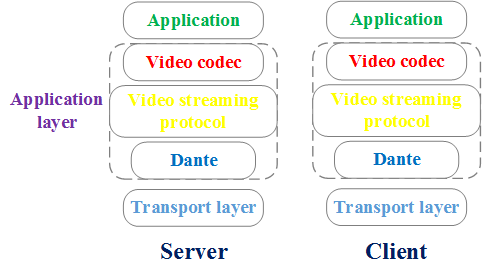
\includegraphics[scale=0.4]{paper_figs/stack_dante.png}
	\caption{Illustration Of Dante}
	\label{paper_figs:pathdemo}
\end{figure}

\begin{figure}[ht]
	\centering
	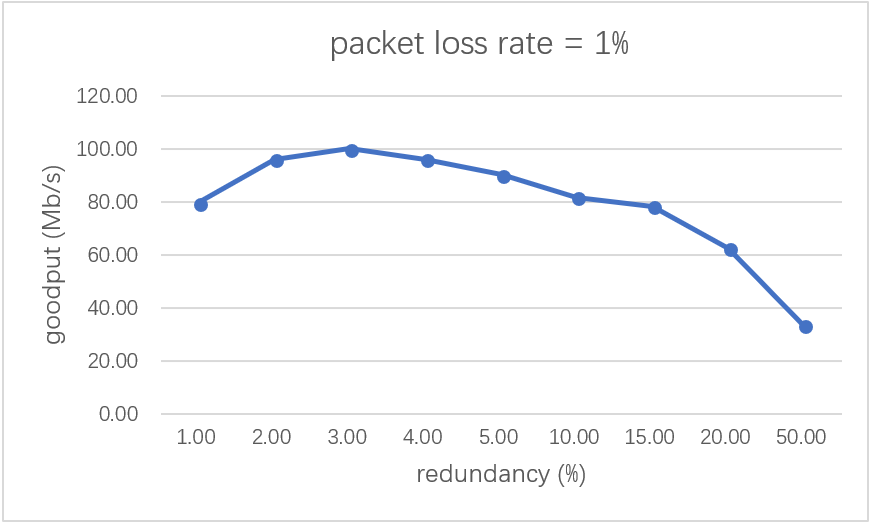
\includegraphics[scale=0.25]{paper_figs/tradeoff_only_goodput.png}
	\caption{The Goodput When Increasing The FEC Redundancy}
	\label{paper_figs:pathdemo}
\end{figure}


\tightsection{Introduction}

% 360 degree videos are important
360-degree videos are coming to age, largely driven by content
providers (\eg CNN, New York Times) serving more immersive content (\eg 
NBC broadcasting the 2018 Winter Olympics in VR~\cite{NBC_olympic_360}), 
as well as 
by more immersive video 
devices~\cite{google_developers,facebook360,SUMSUNG_HEADSET}.
However, streaming 360-degree videos to mobile devices over wireless
networks remains a substantial challenge.

% why it's challenging
To offer true immersive experience, 360-degree videos must be streamed
in high resolution and within a small, bounded delay.

\begin{packeditemize}
% low delay
\item {\em Stringent delay constraint:} 
To prevent simulator sickness \cite{Simulator_Sickness} and ensure high
video quality, HeadMounted Display vendors recommend that the video systems
react to head movements as fast as the HMD refresh rate.
Given that
refresh rate of state-of-the-art HMDs is 120Hz \cite{120fps},
the whole system should react in less than 10ms.
These stringent delay constraints render many traditional streaming 
techniques (\eg~\cite{MPEG-DASH}) insufficient.

%\jc{reword the last sentence. what's "application round-trip latency"? why "sickness" is caused by some "refresh rate"?} These stringent delay constraints render many traditional streaming  protocols (\eg~\cite{??,??}) insufficient.

% high bandwidth
\item {\em High-bandwidth consumption:}
360-degree videos require high bandwidth in order to stream videos in
high resolution, ideally, over the whole 360-degree sphere; \eg the 
bitrate of an 8K 360-degree video encoded at a frame rate of 60 
frames per second with HEVC~\cite{HEVC} is $\sim$100Mbps. However,
according to
OpenSignal~\cite{opensignal}, almost a half of the 77 surveyed 
countries in 2017 over the world only have access to 4G cellular 
networks of 10-25 Mbps.
\end{packeditemize}
% \vspace{-0.1cm}

% fov-aware streaming & problems
One  common approach to addressing this challenge is that, 
instead of streaming all video content simultaneously, one can stream
only the video content in and around the viewer's FOV,
or prioritize data in those FOV regions over non-FOV regions. This 
FOV-aware approach has attracted great attention in recent 
years~\cite{Viewport-adaptive,360ProbDASH,Adaptive_Streaming_Framework,Two-tier,Omnidirectional_Video_over_HTTP}, 
leading to various strategies that adapt application-level 
parameters, \eg 
encoding bitrate, to allocate bandwidth intelligently 
to ensure good quality of content in the FOV regions. 
However, these application-level strategies 
fail  to directly reduce the streaming delay. This is because 
they run on top of transport mechanisms that rely on 
retransmission to send the video content in its entirety,
and due to long latency in wireless networks and 360-degree video's
stringent delay constraint, any retransmission
can potentially cause playback interruptions.
% existing transport protocols that are unaware of FOVs
% and thus fail to leverage the fact that data packets may have different
% inherent priority depending on whether the carried video data belong to
% FOV region.

% custom transport protocols & problems
On the other hand, there have been proposals of custom transport 
protocols for streaming delay-sensitive videos~\cite{MPMTP,CMT-VR,ADMIT}. 
Unfortunately, they have so far focused on traditional video content, 
as opposed to 360-degree videos. So the opportunities of developing a 
custom transport protocol for 360-degree video streaming remain untapped.
In particular, when setting the transport-level actions (\eg redundancy
levels), they fail to leverage the spatial heterogeneity of 
viewer's attention around FOVs.

% our solution
In this paper, we propose {\em Dante}, an FOV-aware transport protocol
for 360-degree video streaming, as depicted in Figure. ~\ref{fig:stack}. 
% Figure. 2 puts Dante into the perspective of previous efforts. 
At the core of Dante are two ideas. First, like other video-specific custom streaming protocols, Dante does not enforce
total reliability which could lead to excessive re-transmissions and 
unstable streaming delay, 
and Dante uses Forward Error Correction (FEC) to recover data losses 
without retransmissions, thus significantly reducing and 
stabilizing the streaming delay.
While these protocols might cause small fraction of missing frames 
(except key frames for which we do apply retransmission to ensure 
reliability), our evaluation shows that its impact on video quality is 
negligible, even under highly lossy network connections. 
Second, Dante prioritizes FOV regions by using more FEC redundancy to 
send data packets belonging to FOV regions (predicted by the 
video player). This effectively gives packets in FOV regions more 
bandwidth, higher reliability, and more chance to meet the streaming 
delay constraint.

We use two videos downloaded from Youtube as our dataset to 
evaluate Dante and compare it with TCP-based 360-degree streaming 
protocols, FOV-aware DASH \cite{Omnidirectional_Video_over_HTTP} and traditional FEC-enabled streaming protocols MTMTP \cite{MPMTP} and CMT-VR \cite{CMT-VR} 
that are not FOV-aware. The experimental results show that Dante 
improves video PSNR over current video transport protocols by
20\% to 30\%. Furthermore, Dante, combined with FOV-aware tile-based bitrate adaptation, improves video PSNR over TCP-based FOV-aware DASH by 40\%.
%\jc{how about TCP-based?}

%\jc{need a para to summarize the key results: 
%we use what dataset to evaluate the performance of Dante and compares it against what baseline.  the experimental results show that Dante improves what metrics over  what baselines by how much}




% \section{Background And Motivation}

	Generally, VR headset has a 110 degree horizontal FOV and a 90 degree vertical FOV, and the fraction of videos of video which extracted and displayed on HMD anytime would be $\frac{{110^\circ }}{{360^\circ }} \times \frac{{90^\circ }}{{180^\circ }}{\rm{ = }}15{\rm{\% }}$. Obvious, the data of the FOV region, viewed by users, is more important than non-FOV region.
	From the perspective of application layer, the FOV-aware tile-based streaming schemes, based on Dynamic Adaptive Streaming over HTTP (DASH), suggests that, 360-degree videos are split and encoded into multiple tiles spatially, each of which can be independently decoded, stored into a single file. Furthermore, according to the distance from the expected viewpoint of users, 360 videos would be split into two or three regions spatially, each of which would be composed of multiple contiguous tiles and store into a single file, as depicted in Figure 3.
	
	\begin{figure}[ht]
		\centering
		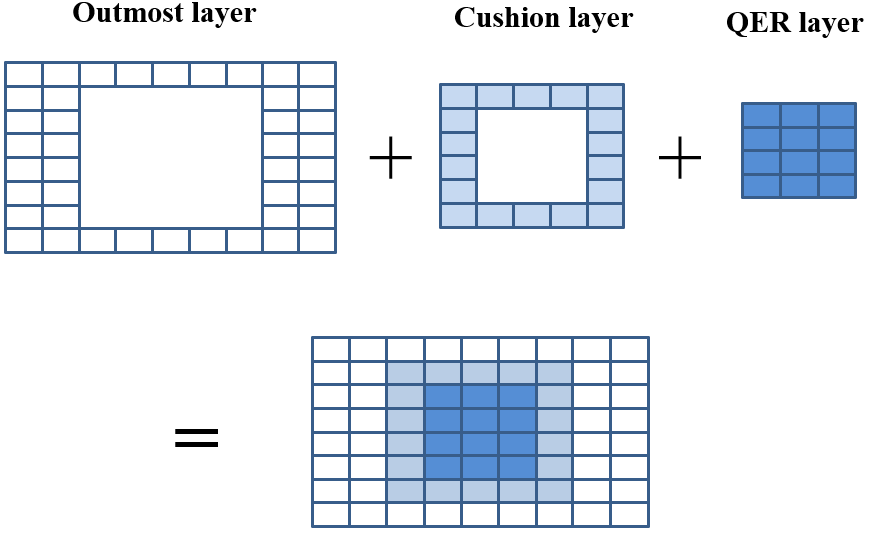
\includegraphics[scale=0.2]{paper_figs/tileSplit.png}
		\caption{360-degree Video Representation}
		\label{paper_figs:pathdemo}
	\end{figure}	
	
	
	However, the state-of-the-art transport schemes, which are not FOV-aware, spend as same amount of bandwidth on reliable delivery of trivial data, i.e., the non-FOV data, as the FOV data. So, can we, from the perspective of reliability of transport, design a protocol, which prioritizes the reliability of FOV data over non-FOV data, boosting the whole system performance by sacrificing little degree of quality of non-FOV data.

    
	Instead of only retransmissions, FEC\footnote{In Dante, FEC is generated through erasure coding of blocks of packets, to recover lost packets, which should be distinguished from FEC, computed on individual packets using channel coding, recovers from bit errors.} is adopted to be a proactive scheme of reliability in our proposed protocol. It can achieve low delay by mitigating retransmissions and is generally be in favoured by real-time video services. However, how to adjust the degree of FEC redundancy is a challenging problem. 
	 
	For example, considering a chunk of data organized into K packets, with equal length, the FEC encoder takes the K data packets, and adds A repair packets to create a coded block of size ${\rm{B = (K + A)}}$. The receiver can recover completely the origin data of $K$ packets if any not less than $K$ packets of all ${K + A}$ packets are received. The code rate is equal to ${K/B}$ and the redundancy of FEC is ${(A/K)}$ . Obviously, it can recover $A$ packets of loss over lossy links at most and when FEC redundancy packets is more, the coding system has more powerful recoverability. 	 
	
    Increasing FEC redundancy can improve recovery probability of data packets in order to mitigate the degradation of video quality caused by packet transmission loss. However, with the increasing of redundancy and computing overhead of coding \cite{ASCOT}, the over-provisioning of redundancy may enlarge end-to-end delay, even causing unnecessary data loss caused by the hit of deadline. As depicted in Figure 2, with the increment of FEC redundancy, while the original data can be recovered with higher probabilities, the goodput first goes up to a peak point and degrades  latter, gradually. So, it's important to carefully adjust the redundancy of FEC in order to balance the tradeoff between recovery probability and goodput performance.  
	 
	We temporarily consider the situation where the video is split into two region, FOV region and non-FOV region. We find, instead of different regions encoded with the same FEC redundancy, it can lead to the better video quality that different regions are encoded with different FEC redundancy before the transmission. 
	 
    For example, the network status is set where average packet loss rate is set to 1\%, bandwidth is set to 40Mb/s. Meanwhile, the length of video segment is equal to o.5s, the size of FOV region is selected into 4Mb, the size of non-FOV region is 20Mb and playback deadline is set to 500ms. As illustrated in Table 1, while the set where all regions is encoded wih the same redundancy, perform worse among them the combination, the redundancy of FOV region and non-FOV is 2\% and 5\%, respectively, achieves obvious upgrade of video quality in FOV, and little degradation of video quality in non-FOV. Furthermore, FOV data, which is more likely perceived by users, is more important to QoE of video than non-FOV and the whole video quality is boost. So, when the network is limited-source and error-prone, if carefully designed, the schemes in which systems prioritized FOV data over non-FOV data, i.e., reliability VS best-effort, can effectively boost the whole system performance.       
	
	\begin{table}
		\centering 
		\scriptsize
		\begin{tabular}{p{2.0cm}p{2.0cm}p{1.6cm}p{1.6cm}}
			\rowcolor[gray]{0.9} 
			\hline
%			 The length of segment &The size of QER region(Mb) & The size of non-QER region(Mb) &
			The FOV redundancy(\%) &The non-FOV redundancy(\%) & Expected PSNR of FOV(dB) & Expected PSNR of non-FOV(dB)\\
			\hline
			3  &  3  &  35  &  35\\    
			\hline
			2  &  5  &  43  &  33\\ 
			\hline
			
		\end{tabular}
		\caption{The Video Quality of different FEC redundancy combinations}
		\label{}
	\end{table}
	 
	 
	Based on the above observations, unlike the 360-degree tile-based streaming schemes, which perform FOV-aware bit-rate adaptation on different region, we proposed Dante, the reliability scheme of which performs on different region of videos in a hierarchical fashion, i.e, preferentially provisioning the data closer to FOV with more FEC redundancy. Thus, the data, which more strongly affects QoE of video, transmitted over lossy links, is supposed to integrally received with a higher probability and thus QoE of 360-degree video can be boosted notably.
 
%Meanwhile, in Table 1, we summarize the main differences of Dante with the existing multipath schemes. 
To the best of our knowledge, Dante is the first FOV-aware 360-degree video protocol over heterogeneous wireless networks.






%\subsection{360-degree Tile-based Streaming}

%%In order to mitigate dependence on high bandwidth, FOV-aware tile-based streaming scheme, based on Dynamic Adaptive Streaming over HTTP (DASH) \cite{MPEG-DASH}, is extensively studied in recent years. For most typical works~\cite{Viewport-adaptive}\cite{360ProbDASH}\cite{Adaptive_Streaming_Framework} \cite{Two-tier}\cite{Omnidirectional_Video_over_HTTP}\cite{Furion}, 360-degree videos are split into segments of equal length, such as 1s, and the server offers multiple bit-rate of representations for every segment. Furthermore, with the technology of motion-constraint tile sets (MCTS), every segment can be encoded into multiple tiles spatially, as depicted in Figure 1, each of which can be independently decoded, stored into a single file and sent to clients alone. So, the server offers representations that also differ spatially by having a Quality Emphasized Region (QER)~\cite{Viewport-adaptive}: a region of the video which is made up of tiles with higher bit-rate than the rest of tile of the remaining of the video. Clients periodically pre-fetch a representation for the next segment such that the bit-rate adapts to available bandwidth and QER best matches the expected viewport of users.
%Unfortunately, these state-of-the-art works~\cite{360ProbDASH} \cite{Adaptive_Streaming_Framework} \cite{Two-tier} \cite{Omnidirectional_Video_over_HTTP} \cite{Furion}, which focus on the delivery of 360-degree video and only solved the problem of FOV-aware bit-rate adaptation in application layer, failed to design a effective FOV-aware scheme to guide the transport protocol to counter limited bandwidth and time-varying problem in mobile scenarios. 
%For example, they still use HTTP, built on top of TCP, as their transmission protocol. which, however, coupling flow and congestion control, suffers from poor throughput and delay performance in wireless networks featured by high loss rate, is inappropriate for 360-degree video delivery.

% Unfortunately, they only strive to optimize FOV-aware bit-rate adaptation schemes in application layer and failed to consider a effective FOV-aware scheme to guide the transport protocol. Thus, they can not perform well over lossy links, even worse in mobile scenarios.  

%However, even combined with 360-degree tile-based streaming, due to the failure to consider FOV, 

%\subsection{The introduction of FEC}
%	 MultiPath Parallel Transmission, considering mobile devices, like smartphone, almost equipped with diffrent radio interfaces (eg.Wi-Fi and LTE), is considered to be a promising way to solve the problem of limited bandwidth over wireless links. IETF-MPTCP \cite{IETF-MPTCP} is proposed and suffers from the performance degradation subject to the bottleneck link. These works~\cite{MPLOT}\cite{FMTCP} \cite{HMTP}, due to the introduction of FEC and well designed data allocation algorithm, not only aggregate capacities across paths but counter wireless network's time-varying characteristic, mitigating the head-of-line blocking and packet out-of-order in multiple diverse network.
\tightsection{Motivation}

We first motivate the two key ideas of Dante:
(1) reducing streaming delay by replacing today's 
TCP-based streaming with retransmission-free FEC-based streaming, and 
(2) further improving quality using FOV-aware FEC coding.


\begin{figure}[t!]
	\centering
	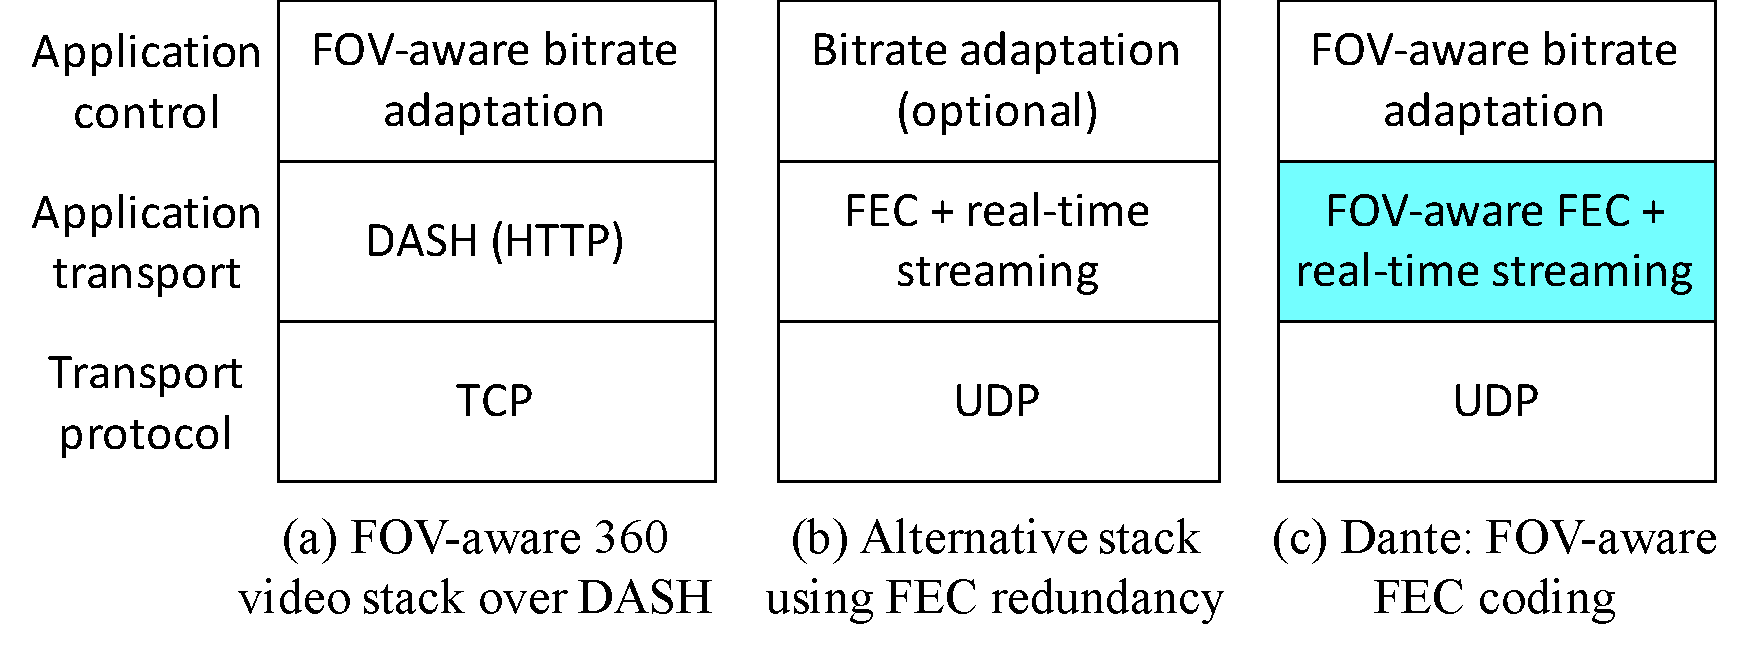
\includegraphics[width=0.5\textwidth]{paper_figs/dante-stack-comparison.pdf}
	\vspace{-0.5cm}
	\tightcaption{Contrasting Dante with previous solutions. 
	Dante proposes to replace the TCP-based streaming stack with 
	UDP-based FEC-enabled streaming stack to improve timeliness of 360-degree videos,
	and proposes to use FOV-aware FEC coding to further improve 
	delay-quality tradeoffs. 
	%\jc{This figure is still missing!!}
	}
	\label{fig:stack}
\end{figure}

We start with some background on 360-degree video streaming and 
the recent related work. In basic 360-degree video streaming, the 
server first encodes the video into 360-degree frames using standard 
video codecs (\eg HEVC~\cite{HEVC}) and streams them over TCP to the 
video player, which then plays the video in the region that the viewer
is currently watching, \ie FOV. Of course, this 
naive scheme works poorly in bandwidth-limited and error-prone 
wireless networks, because the available bandwidth can be less than 
what is needed for sending the 360-degree frames in their entirety. 


To address this issue, many recent work ~\cite{Viewport-adaptive,360ProbDASH,Adaptive_Streaming_Framework,Two-tier,Omnidirectional_Video_over_HTTP,Furion} propose 
to spatially partition each 360-degree frame to fine-grained 
``tiles'' (illustrated in Figure~\ref{fig:tile-based}), 
so that any FOV
of a viewer can be played by sending 
a small subset of tiles that cover the FOV, rather than the whole 
360-degree frame. This greatly saves bandwidth consumption. For 
instance, an FOV area typically spans 110 degrees horizontally and 
90 degrees vertically, so the fraction of video needed to cover FOV 
area is $\frac{{110^\circ }}{{360^\circ }} \times 
\frac{{90^\circ }}{{180^\circ }}{\rm{ = }}15{\rm{\% }}$ 
of the original 360-degree video. To leverage this observation, a 
common approach is to encode each tile in multiple bitrates, and in 
play time, the player predicts the FOV area and requests the tiles 
in different bitrate depending on how likely each tile falls in the 
FOV area. 

\begin{figure}[t]
		\centering
% 		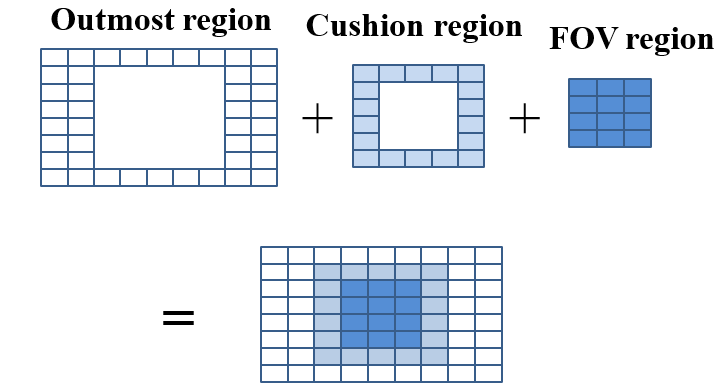
\includegraphics[scale=0.34]{paper_figs/tile_3_regions_0626.png}
        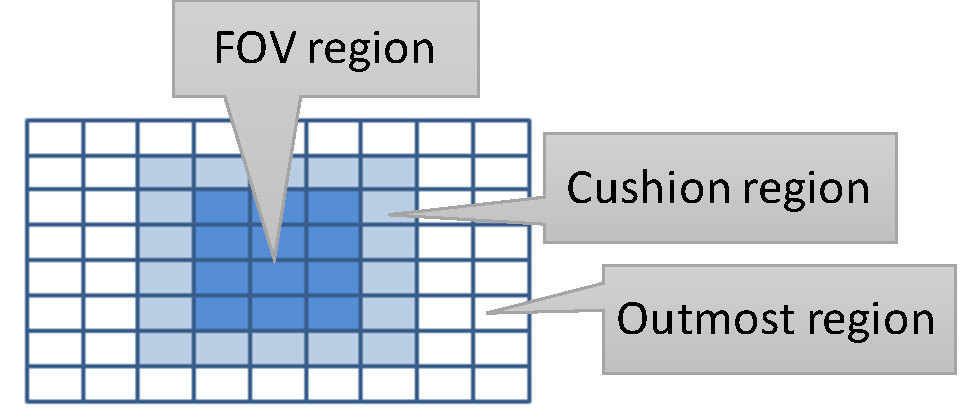
\includegraphics[scale=0.34]{paper_figs/dante-representation.pdf}
		\tightcaption{Tile-based representation of 360-degree video. Video 
		content in the FOV (field-of-view) region will be prioritized,
		\eg higher bitrate.}
%		\jc{please make it one line? don't call them "layers", call them "regions". }
		\label{fig:tile-based}
\end{figure}


\tightsubsection{Why FEC coding?}

Despite much bandwidth saving, these tile-based bitrate adaptive 
streaming techniques still use TCP (mostly via HTTP as an 
intermediate layer~\cite{MPEG-DASH}), and is ill-suited to streaming 
high-quality content while meeting constant and small streaming 
delay, because TCP is prone to be negatively affected by latency 
jitters and random packet losses, potentially causing interruptions
in video playbacks. Interruptions can cause viewers of 360-degree 
immersive videos to feeling dizzy~\cite{Simulator_Sickness}, 
so 360-degree videos are much more sensitive to 
playback interruptions than of traditional video content. The FOV-aware adaptive streaming schemes require system to prefeatch the video segment. However, it is difficult to accurately predict user's orientation
especially for long-term prediction (> 3s) \cite{360cellular}. Hence, the buffer length should be not greater than 3s so as to guarantee the quality of the video fraction users are actually watching.


%\jc{add some concrete numbers on how much short the latency needs to be and provide citations/references. }

Instead of using retransmission to provide reliability, we consider
an alternative approach that uses FEC 
code to deliberately introduce a controlled amount of redundancy, so 
that a small number of packet losses can be recovered without 
retransmission. FEC-enabled protocols (\eg RTP~\cite{rfc5109}) are often 
used to support delay-sensitive video streaming over UDP
(\eg video conference). 

The basic idea behind using FEC in video streaming is as follows. 
If a video segment includes $K$ uniform-sized data packets, the FEC 
encoder then takes these packets as input and adds $A$ ``repair 
packets'' to create a coded block of size ${{B = K + A}}$. And we assume the packet size is equal to Maximum Transmission Unit (MTU). These redundant repair packets allow the receiver to recover the origin $K$ packets, as long as at least {\em any} $K$ of the ${K + A}$ 
packets are received.\footnote{It is worth noting that the FEC in 
this paper operates at the level of data packets, rather than bits.
That is, we do not add redundancy to each individual packet (as in 
some link-level protocols); instead, we apply FEC coding to 
generate redundant packets of a given group of packets to tolerate
any packet-level losses.} The redundancy of FEC is defined by 
${A/K}$. Obviously, one can tolerate more packet losses by using a 
higher FEC redundancy. 
%\jc{make sure the math notions, B, K, A are not used in other sections, or are used with the same physical meaning}
	
A critical question is whether the benefit of FEC coding (\ie less
latency) outweighs its cost (\ie increased data sizes).
Figure~\ref{fig:goodput_redundancy} shows the impact of the FEC redundancy on the video
streaming goodput---the amount of video data (after FEC decoding) 
received within a fixed delay (1s) after it is sent out. The network parameter set is seen in section 4.
%\jc{what's the set up here? you can add a forward pointer to eval if it's the same set up you will explain there. what data was used to generate the graph? what's the delay constraint? how was the network condition (pkt loss rate, delay)?}
As FEC redundancy increases, at first the goodput 
does increase, since a bit redundancy improves robustness against 
packet losses. The goodput peaks at FEC redundancy of 3\%,  and then begins to
drop with higher FEC redundancy, 
as too much redundancy starts to cause self-inflicted congestion.
The important takeaway here is that setting a suitable value of FEC 
does improve video streaming quality by striking the balance between
robustness against packet losses and throughput. 

\begin{figure}[t]
	\centering
	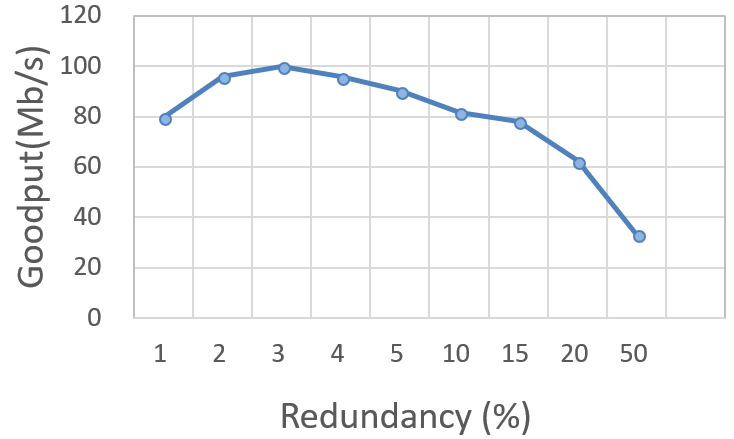
\includegraphics[scale=0.32]{paper_figs/goodput_With_redundany_big_font.png}
	\tightcaption{The impact of various FEC redundancy on video streaming goodput.}
	\label{fig:goodput_redundancy}
\end{figure}


\tightsubsection{Why FOV-aware FEC?}
By replacing the TCP-based streaming protocol in 360-degree videos 
with UDP-based and FEC-enabled protocols, we not only reduce 
streaming delay, but 
introduce a new opportunity as well---one can further improve 
FEC-enabled streaming protocol by taking advantage of the 
fact that the viewer's attention is not uniformly spread, 
but focuses on FOVs.

Figure~\ref{fig:example} 
shows an example of this opportunity in action. We
consider two spatial regions in the same 360-degree video segment, 
one in the FOV region, and the other in the non-FOV region, and we use 
two strategies to set FEC redundancy, one unaware of FOV (giving 
equal FEC redundancy to both regions) and the other aware of FOV (\ie 
giving a better FEC redundancy to the FOV region than the non-FOV 
region). In this example, we set packet loss rate to be 1\%,
network capacity 40Mb/s, video segment length 0.5 second, the delay constraint is 500ms, i.e., the video segment should be encoded by FEC encoder of the server side, then sent, received and finally decoded by FEC decoder of the client side within 500ms, the size of FOV region
4Mb, and the size of non-FOV region 2Mb (\eg application assigns 
a lower bitrate to the non-FOV region, but this doesn't affect our 
observation). We use PSNR ~\cite{Viewport-adaptive} to measure the video quality by calculating the effect the noise caused by information loss has on video fidelity. The higher is video's PSNR, the better is it's quality. 
%\jc{how exactly this is done?}
Now, compared to applying FEC redundancy of 3\% to both regions, 
if one apply 5\% to the FOV region and 2\% to the non-FOV region, 
the resulting video quality in the non-FOV region will be almost the 
same (with a marginal 5.7\% drop), but the video quality in the
FOV region is significantly improved by 23\%. 
Note that 23\% is a significant improvement,
given PSNR is in log scale. 
%\jc{say something like: 23\% is significant because psnr is in log scale, etc}
%\jc{what does 23\% higher PSNR mean physically? can you find some quote? 我查了相关的文献,暂时没有找到具体的解释}

% We find that, instead of different regions encoded with the same 
% FEC redundancy, it can lead to the better video quality that 
% different regions are encoded with different FEC redundancy 
% before the transmission.

\begin{figure}[t!]
	\centering
	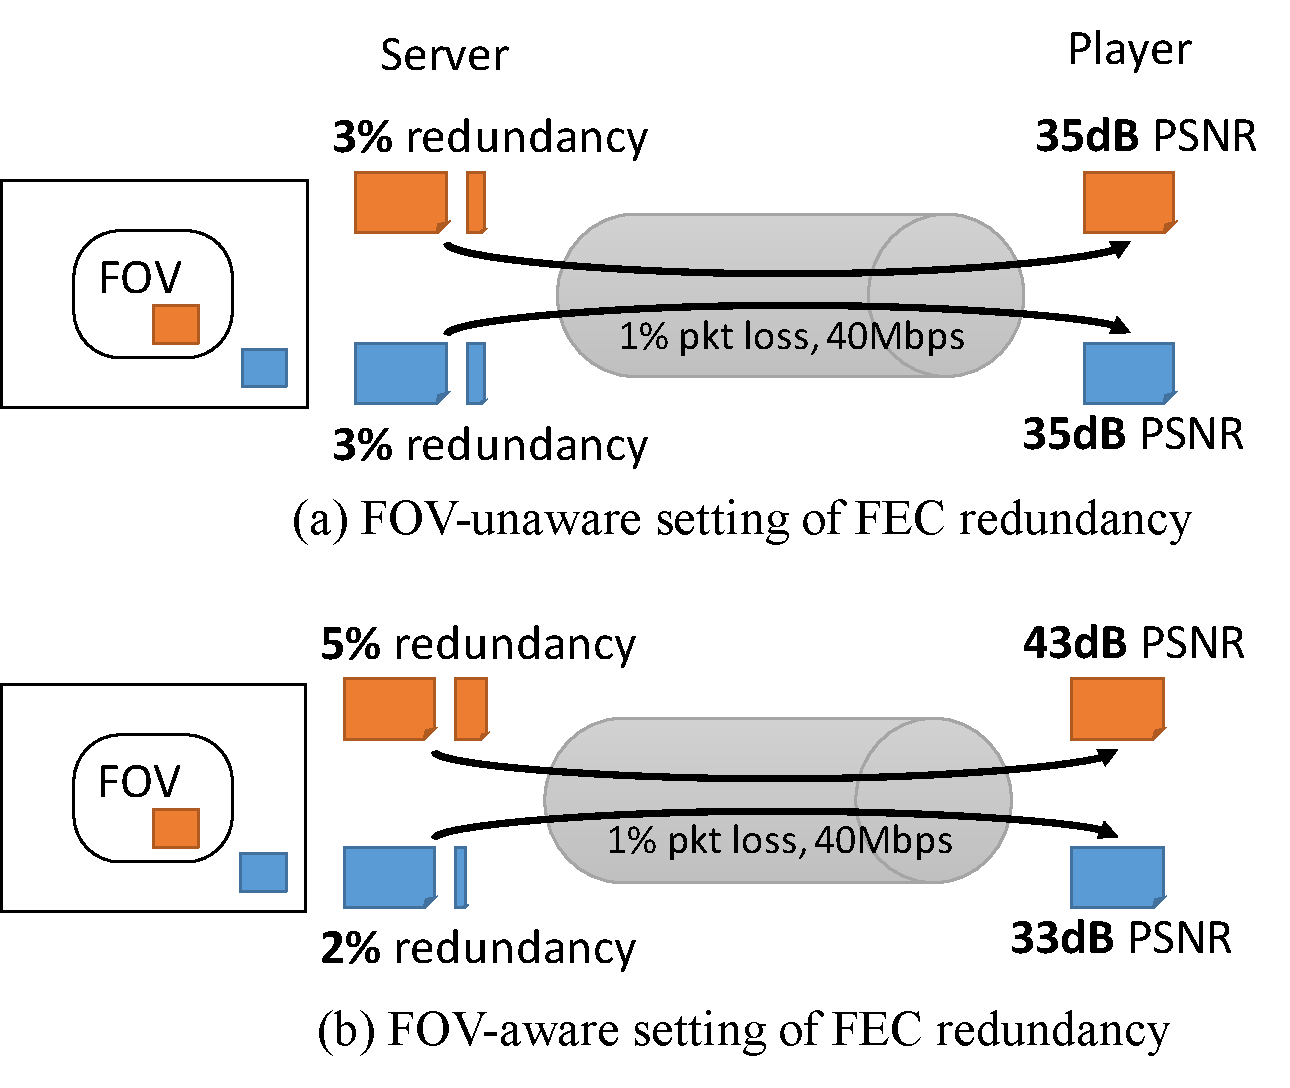
\includegraphics[width=0.36\textwidth]{paper_figs/dante-fec-example.pdf}
	\tightcaption{An illustrative example that setting FEC redundancy based on FOV can significantly 
	improve video quality in the FOV regions.}
	\label{fig:example}
\end{figure}
	
% 	\begin{table}
% 		\centering 
% 		\scriptsize
% 		\begin{tabular}{p{2.0cm}p{2.0cm}p{1.6cm}p{1.6cm}}
% 			\rowcolor[gray]{0.9} 
% 			\hline
% %			 The length of segment &The size of QER region(Mb) & The size of non-QER region(Mb) &
% 			The FOV redundancy(\%) &The non-FOV redundancy(\%) & Expected PSNR of FOV(dB) & Expected PSNR of non-FOV(dB)\\
% 			\hline
% 			3  &  3  &  35  &  35\\    
% 			\hline
% 			2  &  5  &  43  &  33\\ 
% 			\hline
			
% 		\end{tabular}
% 		\caption{The Video Quality of different FEC redundancy combinations}
% 		\label{}
% 	\end{table}

% Finally, note that our approach is complementary to the 
% application-layer tile-based bitrate adaptation: given any 
% selection of tile and bitrate, we apply FEC coding to improve
% timeliness of streamed content by avoiding resending data 
% packet as in TCP.

% 
\section{Protocol Design}
Unlike the video bit-rate adaptation of FOV-aware streaming, Dante, from the perspective of reliability scheme, preferentially provisions the tiles, which are viewed by user with higher probability and are more important to user's QoE, with more FEC redundancy.  

%We consider the expected video quality loss caused by transmission loss and decoding dependencies of video codec, both of which depend on the FEC parameter adjusting procedure.	

\subsection{FEC Redundancy Adaptive Adjusting}
The aim of FEC adaptation is to find the optimal FEC redundancy for different data. The key to achieve this is how to judge whether a kind of FEC redundancy is optimal. Obviously, the optimal FEC redundancy is obtained when best QoE of videos is achieved.  video distortion can be considered as a standard metric of QoE. 

\subsubsection{optimization problem}

we consider that optimal FEC redundancy is obtained if minimization of the video distortion is achieved.
Given predicted viewing probability distribution, packet loss rate $\Pi _m^\alpha$, the optimal FEC redundancy for each layer of all frames can be obtained by solving the following optimization problem, which can be formalated as:
\begin{eqnarray}
&{\{ R_m^a\} _{1 \le m \le M,a \in Q}} = \arg \min (\sum\limits_{i = 1}^M {d_{m,effective}}).  \\
&{\rm{subject}}{~~\rm{to}}{~~~T^{tran}} \le {T_{GOP}}~~~~~~~~~~~~~~~~~, \\
&{\rm{and}}{~~~~~~\lambda ^p}(\Phi ) \le {\mu _p}\begin{array}{*{20}{c}}
{}
\end{array}{\rm{}},{\rm{}}~~~~~~~1 \le p \le P~~~,\\
&\begin{array}{*{20}{c}}
{{T^{tran}}{\rm{ = }}}&{\frac{{\sum\nolimits_{m = 1}^M {\sum\nolimits_{\alpha  \in Q} {(V_m^\alpha  \cdot (1 + R_m^a))} } }}{{t{r^{TFRC}}}}}
\end{array},\\
&{\lambda ^p}(\Phi ) = \lambda \frac{{\sum\nolimits_{m = 1}^M {\sum\nolimits_{\alpha  \in Q} {{{(V_m^\alpha  \cdot (1 + R_m^a))}_{_{\left\{ {\Phi _m^\alpha  \in p} \right\}}}}} } }}{{\sum\nolimits_{m = 1}^M {\sum\nolimits_{\alpha  \in Q} {V_m^\alpha } } }}.
\end{eqnarray}

Where, the minimization of distortion for every GOP is the goal of our protocol's FEC parameters adjusting, subject to constraints of deadline and available bandwidth. And $\{ R_m^\alpha \}$, denotes the redundancy of the $\alpha$ layer for the m-th frame. The first constraint (Eq. (3)) indicates that, due to video's timeliness, the data of every GOP should be transmit to the client side before the delay constraint $T_{GOP}$.
Menwhile, ${V_m^\alpha }$ denotes the size of the $\alpha$ layer for the m-th frame. Given the packet size, S, the estimated round trip time, RTT and estimated packet loss rate, $\Pi_m^\alpha$, the tranmission time of GOP can be calculated by this procedure that the size of GOP, already considering the introduction of FEC redundancy, is divided by the transmission rate, $t{r^{TFRC}}$, according to \cite{TRFC}. 

$\Phi$, a vector, denotes the result of packet scheduling in the scheme of \cite{MPMTP}, which is composed of $\Phi
_m^\alpha {\rm{\{ }}\alpha  \in Q,1 \le m \le M{\rm{\} }}$,  imposed on the $\alpha$ layer for the m-th frame. And the value range of each $\Phi _m^\alpha $ is the serial number of available paths, like 0 to 1.










\subsubsection{Objective funtion And Video Distortion Description}

%So, we design a distortion-driven FOV-aware FEC adaptation.

By comparing the expected value of estimation of video distortion after FEC redundancy provisioning, we can get the optimal FEC redundancy, corresponding to the optimal expected value of distortion. 

Generally, PSNR is used to evaluate the video quality which is calculated via Mean Squared Error (MSE). So, we measure the video distortion using MSE. 

According to \cite{distortion_model} and \cite{CMT-VR}, 
The distortion of the m-th frame for every video GOP (group of pictures) can be formulated as:${d_m} = d_{m,trunc}(R_m,\pi) + {d_{m,drift}}$.
However, unlike non-360-degree videos, only a small portion of 360-degree videos spatially is perceived by users anytime. Meanwhile, according to 360ProbDASH\cite{360ProbDASH}, each tile of 360-degree videos requested by users, is expected to be watched by users with a probability following Gaussian Distribution at any time. So we customize the traditional distortion model into the expected value of distortion, called as the effective distortion, which can be calculated in this schemes in which the distortion of each region is multiplied by its probability of viewing. As a result, for each video frame, the effective distortion is formulated as:
the distortion is formulated as following:\[{d_{m,effective}} = \sum\limits_{\alpha  \in Q} {{\gamma ^\alpha }(d_{_{m,trunc}}^{^\alpha } + d_{_{m,drift}}^{^\alpha })} \]
where Q denotes the layer set of 360-degree videos, which includes FOV layer, cushion layer and outmost layer, as depicted in Figure 3. And ${\gamma ^\alpha }$ denotes the accumulated viewing probability of the $\alpha $
layer:
\begin{equation}
{\gamma ^\alpha } = \sum\limits_{i = 1}^{{\Omega ^\alpha }} {{p_i} \cdot
	{S_i}}
\end{equation}
Where ${p_i}$ stands for viewing probability of the i-th tile in the $\alpha $
layer,   ${S_i}$ denotes spherical area of the i-th tile and
${\Omega ^\alpha }$ denotes tiles set of the corresponding layer. 

Obvious, the tiles of FOV, which are viewed by users with higher probabilities, are attached with greater weights than non-FOV. Thus, improving the distortion of FOV region can bring more performance gain in video distortion than non-FOV region. 

Manwhile, given the estimated packet loss rate $\pi _{m,\alpha }^t$,  $d_{m,trunc}^\alpha$, denotes the expected value of MSE with regard to FEC redundancy provisioning for the $\alpha$ layer of the m-th frame, which is
formulated as:
\[d_{m,trunc}^\alpha (\pi _{m,\alpha }^t) = \widehat \delta _m^\alpha  + \Pi _m^\alpha (\pi _{m,\alpha }^t)\cdot\delta _m^\alpha ,1 \le m \le M\]	

%Given a frame $m$, region $\alpha$, FEC-redundancy rate $k$, and estimated packet loss rate $\pi _{m,\alpha }^t$, $d_{m,\alpha}(k,\pi)$ denotes the expected value of MSE of the frame reconstructed from the packets received before the deadline.


where, $d_{m,trunc}^\alpha$ is proportional to $\Pi _m^\alpha$. And given a frame $m$, region $\alpha$, FEC-redundancy rate $k$, and estimated packet loss rate $\pi _{m,\alpha }^t$,
$\Pi _m^\alpha$ denotes the percentage of lost symbols for the $\alpha$ layer of the m-th frame, which is
formulated as ,
\[\Pi _m^\alpha (\pi _{m,\alpha }^t)  = \left\{ \begin{array}{l}
0,\begin{array}{*{20}{c}}
{\begin{array}{*{20}{c}}
	{}&{}
	\end{array}}
\end{array}if\begin{array}{*{20}{c}}
{\pi _{m,\alpha }^t + (1 - \pi _{m,\alpha }^t)}
\end{array} \cdot \pi _{m,\alpha }^o < \frac{{n - k}}{n},\\
\begin{array}{*{20}{c}}
{\pi _{m,\alpha }^t + (1 - \pi _{m,\alpha }^t)}
\end{array} \cdot \pi _{m,\alpha }^o,\begin{array}{*{20}{c}}
{}&{}
\end{array}{\rm{otherwise}}{\rm{.}}
\end{array} \right.\]

where $(n-k)$ denotes the repair packet of FEC block, and  $\frac{{n - k}}{n}$
stands for tolerant packet loss rate and $\pi _{m,\alpha }^o$ denotes the overdue loss rate. Obviously, $\prod _m^\alpha$ is equal to 0 if the provisioning of redundant packets is sufficient for countering packet drops caused by transmission loss and expired arrival. 



\subsubsection{A Algorithm To Solve The Optimal Problem}

Consequently, it's impractical to derive the optimal solution with polynomial time complexity, and the greedy search is not applicable for real time applications. To solve this problem, we design a fast research algorithm, which complexity is $O(N \cdot M \cdot Q)$, to obtain a sub-optimal solution of FEC redundancy adaptive problem, shown in Algorithm 1. 

\begin{algorithm}[!h] 
	\scriptsize
	\centering 
	\caption{FEC redundancy adaptative algorithm}%算法标题      
	\begin{algorithmic}[1]%一行一个标行号
		\STATE $R = \min (Eq.~(3), Eq.~(4))$ , according to delay constraints, Eq. (3) and
		bandwidth constraints Eq. (4),
		\FOR{$\alpha  \in Q$}  
		
		\STATE Calculate $\gamma ^\alpha$ , according to Eq. (1),
		
		\ENDFOR
		
		\STATE $N = \frac{V}{S} \cdot (1+R)$ 
		
		\FOR{$i = 1{\rm{ }} to {\rm{ }}N$}
		\STATE $index{\rm{ }} = {\rm{ }}0,{\rm{ }}{\Delta _d}{\rm{ }} = 0$
		\FOR{$m = 1{\rm{ }}to{\rm{ }}M$}
		\FOR{$\alpha  \in Q$}
		
		\STATE ${d_{effective}} = \sum\limits_{0 \le m \le M} {\sum\limits_{\alpha 
				\in Q} {{\gamma ^\alpha }(d_{_{m,trunc}}^{^\alpha } + d_{_{m,drift}}^{^\alpha
				})} } $
		\STATE ${N_{m,\alpha }} = {N_{m,\alpha }} + 1$
		\STATE $\Delta  = \left| { - {d_{effective}} + \sum\limits_{0 \le m \le M}
			{\sum\limits_{\alpha  \in Q} {{\gamma ^\alpha }(d_{_{m,trunc}}^{^\alpha } +
					d_{_{m,drift}}^{^\alpha })} } } \right|$
		\STATE ${N_{m,\alpha }} = {N_{m,\alpha }} - 1$
		\IF{$\Delta  \ge {\Delta _d}{\rm{ }}$}
		\STATE $index{\rm{ }} = m,\begin{array}{*{20}{c}}
		{layer}
		\end{array} = \alpha ,{\Delta _d} = \Delta$
		\ENDIF
		\ENDFOR 
		\ENDFOR
		\STATE ${N_{index, layer }} = {N_{index, layer }} + 1$
		\ENDFOR
		\RETURN${\left\{ {{R_{m,\alpha }} = \frac{{{N_{m,\alpha }}{\rm{ - }}{K_{m,\alpha }}}}{{{K_{m,\alpha }}}}} \right\}_{(1 \le m \le M,\alpha  \in Q)}}$
	\end{algorithmic}  
\end{algorithm} 




\subsection{System Overview}

Dante is proposed to support high-quality 360-degree video
streaming service over the wireless network. In Dante, UDP combined with Systematic FEC, RS code, is integrated to provide reliable delivery over wireless networks. And only the data of I frames is retransmitted if no ACK is received by the server in time ${T^I}$, in order to guarateen the video data received is decodable by video codec.
Besides, TCP is supplementary to exchange control information, which is of significance. The overall protocol architecture is illustrated in Figure 2.

\begin{figure*}[ht]
	\centering
	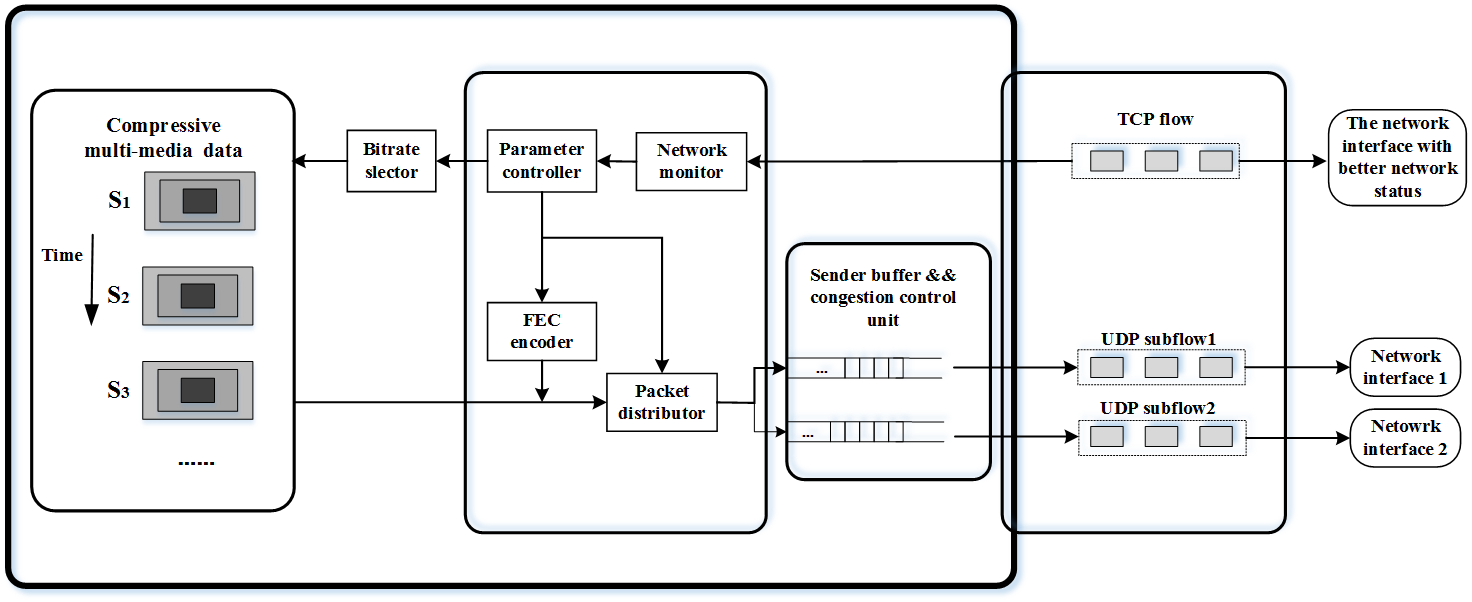
\includegraphics[scale=0.4]{paper_figs/architecture_V2.png}
	\caption{The Architecture of Protocol}
	\label{paper_figs:pathdemo}
\end{figure*}

\tightsection{Design of Dante}

This section presents a detailed system design of Dante.
We begin by formulating the underlying video quality optimization
problem of Dante (\S\ref{subsec:objectives}), and then present a 
simple and efficient control logic that approximately optimizes 
the problem (\S\ref{subsec:logic}), and finally describe a 
prototype implementation of Dante (\S\ref{subsec:impl}) which we
use for evaluation (\S\ref{sec:eval}).

\tightsubsection{Optimization goals}
\label{subsec:objectives}

The high-level goal of Dante is to set the FEC redundancy for
each tile in a given sequence of frames so as to minimize the
average quality degradation of these tiles weighted by the
probability that each tile will be watched by the viewer. 
Dante takes in as input the estimated packet loss rate $p$, 
the sending rate $f$, $m$ frames each having $n$ tiles (we use
$\langle i,j\rangle$ to denote the $j^{\textrm{th}}$ tile of the
$i^{\textrm{th}}$ frame, $0<i\leq m, 0<j\leq n$), the size
$v_{i,j}$ of tile $\langle i,j\rangle$, the probability 
$\gamma_{i,j}$ that tile $\langle i,j\rangle$ will be watched,
and the quality degradation $\delta_{i,j}$ if tile 
$\langle i,j\rangle$ is not recovered, and the maximum delay 
$T$. Then Dante returns as output the FEC redundancy $r_{i,j}$ 
of the $j^{\textrm{th}}$ tile of the $i^{\textrm{th}}$ frame 
($0<i\leq m, 0<j\leq n$). 
Dante's optimization problem can be formulated as following:
\vspace{-0.2cm}
\begin{align}
\textrm{minimize } & \sum_{0<i\leq m}\sum_{0<j\leq n}\gamma_{i,j}d_{i,j}(p,r_{i,j}) \label{eq:obj}\\
\textrm{subject to } & \frac{1}{f}\sum_{0<i\leq m}\sum_{0<j\leq n}v_{i,j}(1+r_{i,j}) \leq T
\label{eq:timeliness}\\
&r_{i,j} \leq 0 \label{eq:positive-redundancy}
\vspace{-0.4cm}
\end{align}
Here, the objective function (Equation~\ref{eq:obj}) is a
weighted sum of the quality degradation over all tiles where 
each tile $\langle i,j\rangle$ is weighted by the probability 
$\gamma_{i,j}$ of it being eventually watched.
Equation~\ref{eq:timeliness} specifies that all the packets
(after encoding redundant packets and the original ones) must 
be sent out before the deadline $T$. 
Dante typically processes all frames in a group of picture 
(GOP) as a batch, in which case 
$T$ is the duration of a GOP. Note that Dante uses 
TCP-Friendly Rate Control algorithm~\cite{TRFC} to compute a
constant sending rate $f$ based on estimated packet loss rate 
and network latency. Finally, 
Equation~\ref{eq:positive-redundancy} ensures the redundancy 
rate is always non-negative.

The key variable here is the quality degradation $d_{i,j}(p,r)$
of tile $\langle i,j\rangle$, if packet loss is $p$ and we use
FEC redundancy $r=\textrm{\# of redundant packets}/\textrm{\# of original packets}$. 
Suppose there are $k$ original packets of a frame, quality
degradation occurs when the lost packets cannot be recovered, 
\ie the number of lost packets $p(r\cdot k+k)$ is greater than
$r\cdot k$, which means $r<\frac{1}{1-p}$. (Note that FEC can
tolerate the loss of {\em any} $r\cdot k$ packet losses.) Therefore, 
\vspace{-0.25cm}
\begin{equation}
d_{i,j}(p,r) = \delta_{i,j}\textrm{, if }r<\frac{1}{1-p}\textrm{; }0\textrm{, otherwise.}\label{eq:degradation}
\vspace{-0.25cm}
\end{equation}

To be more realistic, Equation~\ref{eq:degradation} can be extended
to include one more cause
of quality degradation. Because encoded frames have inherent
dependencies, excessive packet losses can result in quality
degradation on not only one particular frame, but all frames 
whose video decoding depends on it. For instance, losing a ``P'' frame 
will cause all subsequent ``B'' frames, which depend on it, to be lost, even if enough 
of their packets are received. (Note that due to the paramount 
importance of ``I'' frames, we do apply retransmission to 
guarantee the reliability of each ``I'' frame.) To take into 
account the impact of inter-frame dependency on quality 
degradation, we can reformulate quality degradation 
$d_{i,j}(p,r)$ of tile $\langle i,j\rangle$ as a linear 
combination of all previous $d_{i,c}(p,r),0<c\leq i$, \ie
\vspace{-0.25cm}
\begin{equation}
d_{i,j}^{*}(p,r) = \sum_{0<c\leq i}w_{c,i}d_{c,j}(p,r) \label{eq:degradation-new}
\vspace{-0.25cm}
\end{equation}
where $w_{c,i}$ encodes the dependency of frame $i$ on frame $c$. 
More details can be found in~\cite{distortion_model}. 
In the rest of the paper, we use the formulation based on 
Equation~\ref{eq:degradation-new}.




\tightsubsection{Adaptive logic of FEC redundancy}
\label{subsec:logic}


Next, we present Dante's logic that efficiently solves the above 
problem formulation and sets the FEC redundancy of each tile to 
maximize the overall video quality. 

First of all, our problem formulation cannot be
easily tractable. This is because of the non-linearity of 
$d_{i,j}(p,r)$; according to Equation~\ref{eq:degradation}, 
$d_{i,j}(p,r)$ changes sharply depending on whether $r$ is 
greater than $\frac{1}{1-p}$. In fact, we can reduce the problem 
formulation to the ``knapsack problem'' know to be NP-
complete~\cite{NP-complete}. We briefly sketch the 
reduction here. Imagine we have one item for each tile, so in 
total $m\cdot n$ items to be put in a knapsack; if 
$r_{i,j}<\frac{1}{1-p}$ holds for tile $\langle i,j\rangle$, then 
we set the corresponding item to be 0 (\ie not put in the 
knapsack), otherwise, 1 (\ie put in the knapsack). Then our 
minimizer (Equation~\ref{eq:obj}) can be equivalently transformed 
to a maximizer of a linear combination of the binary variables of 
all items, and Equation~\ref{eq:timeliness} can be equivalently 
transformed to a constraint that another linear combination of 
the binary variables must be lower than a threshold. Finally, the 
resulting description---maximizing a weighted sum of some binary 
variables subject to a constraint that another linear combination 
of the binary variables is less than a threshold---is exactly the 
formulation of 0-1 knapsack problem.


\begin{algorithm}[t] 
	\centering 
	\caption{FEC redundancy adaptive algorithm}
	\begin{algorithmic}[1]
	\STATE $B\leftarrow Tf-\sum_{0<i\leq m}\sum_{0<j\leq n}v_{i,j}$  \footnotesize{//Budget of redundant packets}
	\STATE $r_{i,j}\leftarrow 0, 0<i\leq m, 0<j\leq n$  \footnotesize{//Initializing FEC redundancy}
	\WHILE{$B>0$}
		\STATE $\Delta_{max}\leftarrow 0, Tile_{chosen}\leftarrow None$
		\FOR{$i=1,\dots,m$}
			\FOR{$i=j,\dots,n$}
				\STATE $r_{i,j}^{'}\leftarrow r_{i,j}+\frac{1}{v_{i,j}}$ \footnotesize{//Add one redundant packet to tile $\langle i,j\rangle$}
				\STATE $\Delta\leftarrow\gamma_{i,j}d_{i,j}^{*}(p,r_{i,j})-\gamma_{i,j}d_{i,j}^{*}(p,r_{i,j}^{'})$ \footnotesize{//Incremental quality improvement}
				\IF{$\Delta>\Delta_{max}$}
					\STATE $\Delta_{max}\leftarrow\Delta, Tile_{chosen}\leftarrow\langle i, j\rangle$
				\ENDIF
			\ENDFOR
		\ENDFOR
		\STATE $\langle i, j\rangle\leftarrow Tile_{chosen}, r_{i,j}\leftarrow r_{i,j}+\frac{1}{v_{i,j}}$ \footnotesize{//Greedily add the packet to the most needed tile}
		\STATE $B\leftarrow B-1$ \footnotesize{//Reduce budget by one}
	\ENDWHILE
	\RETURN {$r_{i,j}, 0<i\leq m, 0<j\leq n$}
	\end{algorithmic}  
	\label{alg:dante}
\end{algorithm} 

Given that the problem cannot be solve efficiently, we then give 
an heuristic algorithm (shown in Algorithm~\ref{alg:dante}) that 
can solve the problem in linear time and our experimental results 
indicate it results in good performance. The algorithm starts 
with calculating a budget of total number of redundant packets 
$B=Tf-\sum_{0<i\leq m}\sum_{0<j\leq n}v_{i,j}$. Then it greedily assigns 
each redundant packet in the budget to the tile that currently 
maximizes the reduction of quality degradation, \ie 
$\Delta=\gamma_{i,j}d_{i,j}^{*}(p,r_{i,j})-\gamma_{i,j}d_{i,j}^{*}(p,r_{i,j}^{'})$. 
If tile $\langle i, j\rangle$ is chosen, we increment its FEC 
redundancy value by $\frac{1}{v_{i,j}}$ where $v_{i,j}$ is the 
size of the tile. This process continues until we use up all 
redundant packets in the budget.


\begin{figure}[t]
	\centering
	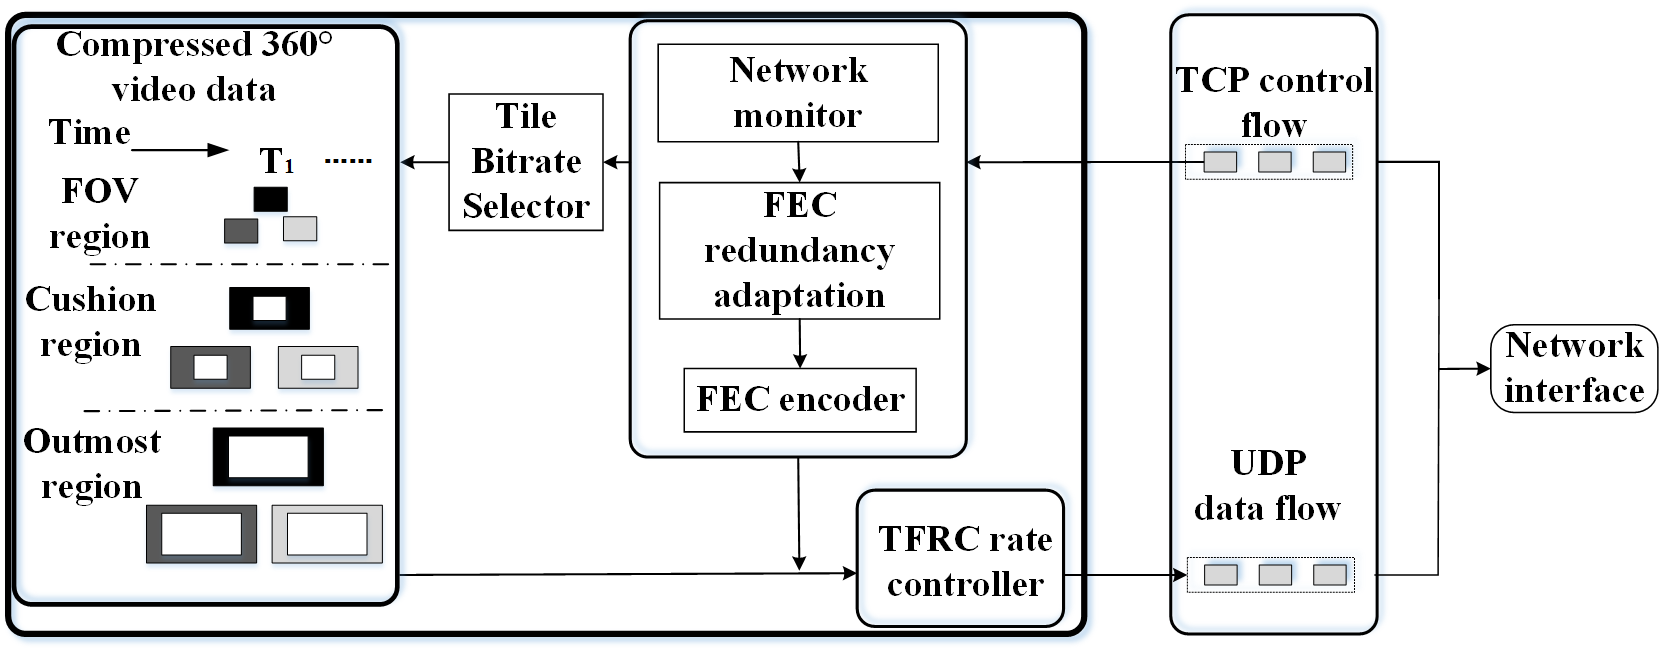
\includegraphics[width=0.5\textwidth]{paper_figs/architecture_dante_0626_v4.png}
	\vspace{-0.3cm}
	\tightcaption{The Architecture of Protocol}
	\label{fig:overview}
\end{figure}




\tightsubsection{Prototype implementation}
\label{subsec:impl}

%\jc{change from client-driven to server-driven!}

We have implemented a prototype of Dante, and here we discuss 
some of its important details. 
Figure~\ref{fig:overview} depicts an overview of the 
implementation. There are two connections between the client and 
the server: one UDP connection to send video data packets, and 
one TCP connection to provide reliable communication of control 
messages, including start/end of a playback session and network information feed (\eg packet loss rate, latency) from receivers. According to the constant network information feed from receivers, the server, at the boundary of each GOP (typically every several seconds), runs Algorithm~\ref{alg:dante} to determine the FEC 
redundancy for the frames and tiles in the next GOP, which then is sent to
 the client. On determining FEC redundancy for frames of the GOP, the server uses 
RS codes to 
inject redundant packets, re-encodes them with the original 
video data packets, and sends the data using TFRC-based sending 
rate. Note that the Dante implementation is complementary to 
application-level bitrate adaptation strategies, and can be 
deployed by replacing the existing underlying transport protocol 
with minimal changes to the video player. 

% Dante is proposed to support high-quality 360-degree video
% streaming service over the wireless network. In Dante, UDP combined with the systematic FEC, RS code, is integrated to provide data delivery service over wireless networks. And only the data of I frames is retransmitted if no ACK is received by the server in time ${T^I}$, in order to guarantee the video data received is decodable by video codec.
% Besides, TCP is supplementary to exchange control information, which is of significance. The overall protocol architecture is illustrated in Figure 2.


% 
%*****Instantaneous PSNR In relatively Bad Network Condition*****	

\begin{figure*}[!t]
	%\begin{figure*}[t]
	\centering
	\subfigure[Video Sequence 1]  {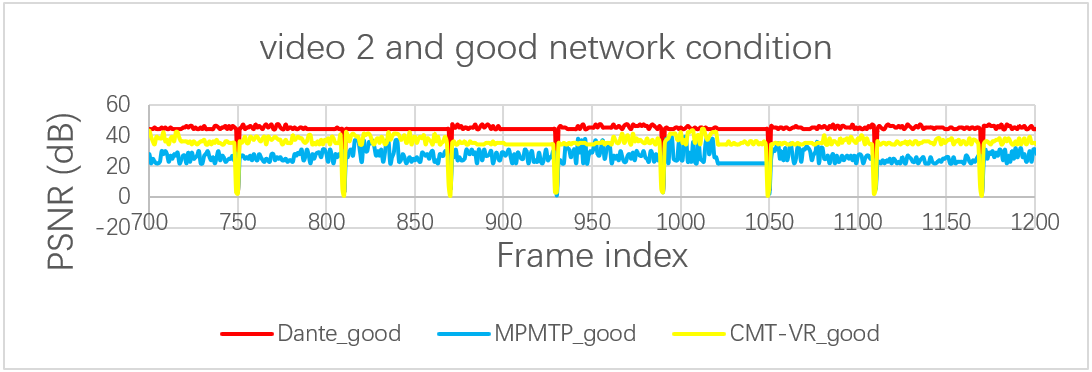
\includegraphics[scale=0.26,angle=0]{paper_figs/evaluation_result/sub/ins_psnr_v2_good.png}}
	\subfigure[Video Sequence 2]  {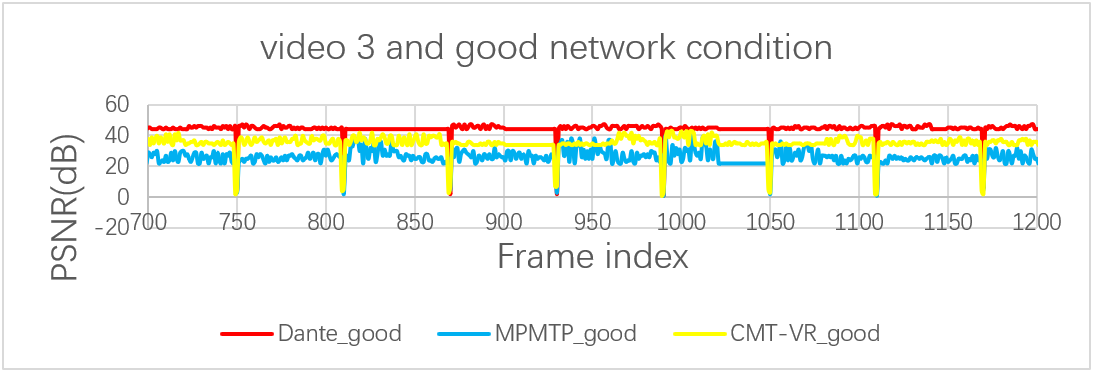
\includegraphics[scale=0.26,angle=0]{paper_figs/evaluation_result/sub/ins_psnr_v3_good.png}}
	\vspace{-0.3cm}
	\caption{Instantaneous PSNR In Relatively Good Network Condition}
	\vspace{-0.4cm}
	\label{fig:apuct}
\end{figure*}

%*****Instantaneous PSNR In relatively Good Network Condition*****
\begin{figure*}[!t]
	%\begin{figure*}[t]
	\centering
	\subfigure[Video Sequence 1]  {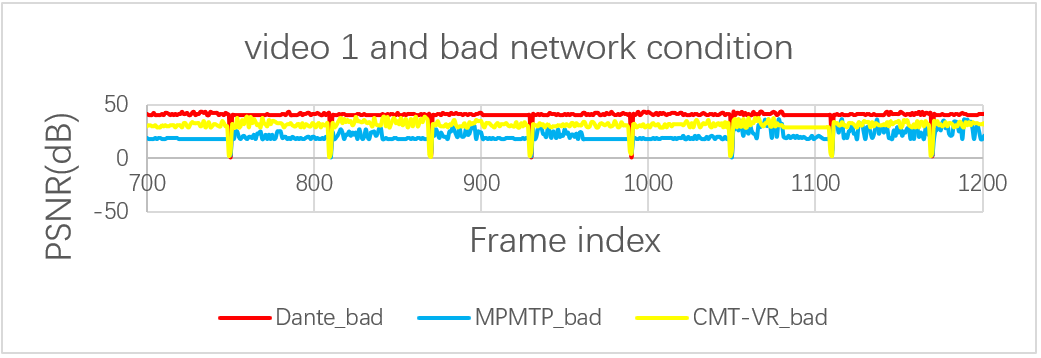
\includegraphics[scale=0.275,angle=0]{paper_figs/evaluation_result/sub/ins_psnr_v1_bad.png}}
	\subfigure[Video Sequence 2]  {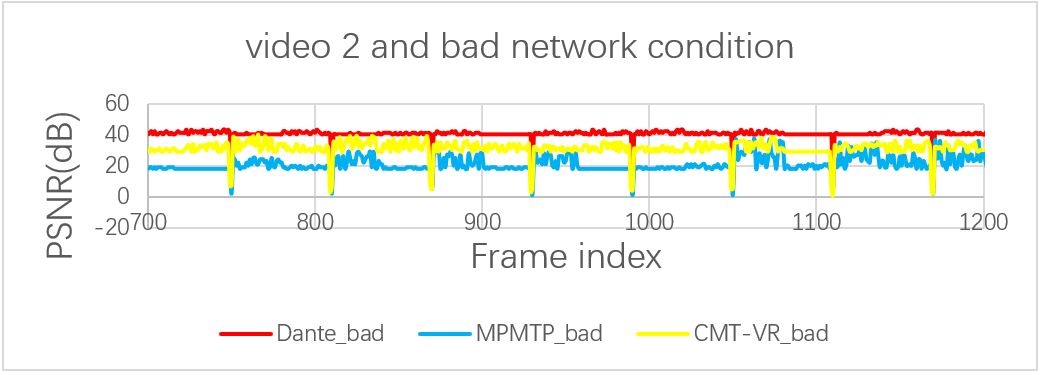
\includegraphics[scale=0.27,angle=0]{paper_figs/evaluation_result/sub/ins_psnr_v2_bad.png}}
	\vspace{-0.3cm}
	\caption{Instantaneous PSNR In Relatively Bad Network Condition}
	\vspace{-0.4cm}
	\label{fig:apuct}
\end{figure*}	




\section{Performance Evaluation}
We use PSNR as the metric of video quality and conducted extensive experiments to demonstrate Dante performance gains on video quality. 

\subsection{Reference schemes}
We evaluate the performance of Dante to compare with two video transport schemes, MPMTP~\cite{MPMTP} and CMT-VR~\cite{CMT-VR}, both of which are not FOV-aware and also utilize FEC to mitigating unnecessary retransmissions. Meanwhile, since the multi-path parallel is not our fous, so we do not take into account these two schemes' path selecting. 
\begin{packeditemize}

\item {\em MPMTP\cite{MPMTP}:} .
This video protocol utilizes the FEC to recover the data,  completely abandoning the retransmission,  in order to maximize the received data rate to prevent playback buffer starvation. This scheme performs in a video content-agnostic fashion. 

% high bandwidth
\item {\em CMT-VR\cite{CMT-VR}:}
CMT-VR, based on SCTP, utilize a quality-driven FEC redundancy  allocation to minimize the distortion of each GOP. Raptor code used to mitigate retransmission. While this scheme considers frame priority, \ie I, P frames, it is in a non-FOV-aware fashion. 

\end{packeditemize}


\subsection{Experimental Set-up}
\textbf{Experiment topology:} The server is connected with the client through one lossy links and Dante is deployed on both server and client side. The topology is not shown because of space limitation. The experiment scenario is that sources send the data to sinks through one lossy links with the request of video data.

\textbf{Testbed configuration:} The sources and sinks are commodity servers with Ubuntu 16.4 (kernel 4.40), each of which is equipped with an Intel(R) Core(TM) i3-4150k cpu @ 3.5GHz (4 cores), one Intel 82599ES 10G dual port NICs and 32 G memory.

\textbf{Parameter sets}
Timeout for triggering I frames' retransmission, $T_I$, is set to 200ms, the size of GOP is set to 15 and the length of video segment, which is request by users each time, is sent to 1s, equal to the time of 2 GOPs. Meanwhile, the size of the receiver buffer is set to 100Mb.
We evaluate the quality of video by computing the expected value of PSNR. So, given a video segment, it's PSNR can be calculated via: \[{V_{PSNR}} = \sum\limits_{i = 1}^{{\Omega ^\alpha }} {({\gamma ^\alpha } \cdot V_{PSNR}^{^\alpha })} \]
where, ${V_{PSNR}^{^\alpha }}$ is the PSNR of the layer $\alpha$. According to a tiles viewing probabilities \cite{360ProbDASH} and (Eq. 7), $\gamma ^\alpha$ can be approximately obtained and $\gamma ^\alpha$ of FOV layer, cushion layer and outmost layer is almost 0.6, 0.3, 0.1, respectively.

\textbf{Network parameter set:} Gilbert model is adopted to mimic the packet loss pattern in real wireless networks, supported by traffic control (TC)~\cite{TC}, in which four parameters($\xi _i^G$, $\xi _i^B$, 1-h and 1-k) are needed, $\xi _i^G$ and $\xi _i^B$ are transition probabilities between the bad and good state, 1-h and 1-k is the loss probability in the bad state and good state, respectively. In our testbed, 1-h and 1-k are set as 1 and 0, respectively. Meanwhile, average packet loss rate is equal to $\pi _i^B = \xi _i^B/(\xi _i^B\\ + \xi _i^P)$. And the bandwidth is also set by TC. The detailed Parameter set is seen in Table 2. 

\begin{table}
	\centering 
	\scriptsize
	\begin{tabular}{cp{1.0cm}p{1.6cm}p{0.8cm}p{2.3cm}}
		\rowcolor[gray]{0.9} 
		\hline
		(A)  &  Time(Sec.)    & Bandwidth(Mbps)       &  RTT(ms) &  Average Pakcet loss rate(\%) \\

		
		&  0${\sim}$60   &  30         &    50    &  0.5 \\

		\hline
		\rowcolor[gray]{0.9}
		\hline
		(B)  &   Time(Sec.)   & Bandwidth(Mbps)       &  RTT(ms) &     Average Pakcet loss rate(\%)  \\
		
		&  0${\sim}$60   &  20         &    50    &  2.5\\
		
		\hline
		
	\end{tabular}
	\caption{Network Condition of Two Wireless networks: (A)Relatively Good Wireless Conditions And (B)Relatively Bad Wireless Conditions}
	\label{}
\end{table}
`
\subsection{Performance Comparison With Existing Protocols}

Then, Figure 5 and Figure 6 compare instantaneous PSNR of three video sequences in good network condition and bad network condition, respectively. The result shows that Dante achieves 20\% to 30\% 360-degree video PSNR performance gain, compared to MPMTP and CMT-VR. The reason why MPMTP performs worst in all protocols is that, despite no involving retransmissions and maximizing the throughput, it doesn't consider video's inherent feature, such as decoding dependencies of video codec, which should have give different frame unequal attention, and thus can't utilize effectively the network allocation to boost video quality. Meanwhile, CMT-VR performs better than MPMTP, due to its consideration of frame priority. However, unfortunately, non-FOV-aware reliability scheme makes it waste valuable bandwidth on trivial data, thus CMT-VR is the secondary one. Dante takes into account not only traditional video features aforementioned, but FOV. Benefiting from the hierarchical protection spatially and temporally, Dante achieves desirable upgrade in instantaneous PSNR. Meanwhile, we find, compared to TCP without FEC, the average CPU time of Dante's, due to the introduction of FEC computing overhead, increases from 14\% to 25\% for the sender side, and from 14\% to 26\% for the receiver side. The overhead of FEC can be ignored considering the performance gain Dante achieves.      
\tightsection{Evaluation}
\label{sec:eval}
We now evaluate Dante's performance and compare it with state-of-
the-art (non-FOV-aware) FEC-enabled streaming protocols as well 
as an FOV-aware TCP-based streaming protocol (DASH).
The main takeaways are two-fold. 
(1) FEC-enabled streaming protocols in general lead to higher 
PSNR than the TCP-based solution.
%, because they can work better 
%under stringent delay constraint. 
(2) By making FEC coding FOV-aware, one can further improve PSNR 
by giving FOV regions more redundancy.


\tightsubsection{Setup}

% We use a server connected with a client through a wireless link with
% controllable loss rate and latency. 
The server and client are 
commodity servers with Ubuntu 16.4 (kernel 4.40), each of which 
is equipped with an Intel(R) Core(TM) i3-4150k cpu @ 3.5GHz (4 
cores), one Intel 82599ES 10G dual port NICs and 32G memory.
They are connected with a lossy link, whose packet loss events are
generated using the Gilbert 
model ~\cite{gilbert_model}. 
Given any average packet loss rate, 
rather than dropping packets uniformly randomly, Gilbert model 
represents the network as a markovian process switching between
two states (high loss rate vs. low loss rate), and picks
the proper transition probability to match the given overall 
packet loss rate. Gilbert model is believed to be more realistic than 
uniform random packet loss~\cite{bernoulli_VS_gilbert}.
%, and uses four 
%parameters---transition probabilities between the two states and 
% the loss rate of each state---to control the overall packet loss 
% rate. So the Gilbert model is believed to be more realistic than 
% uniform random packet loss~\cite{bernoulli_VS_gilbert}. 
We use Gilbert model to generate two 
network traces: one for ``good'' network condition (loss rate $=0.5\%$), and one for
``bad'' network condition (loss rate $=2\%$). 
Table~\ref{tab:parameters} shows the
parameter settings of each trace. 
We use Linux TC~\cite{TC} to control the actual instantaneous loss rate. 

\begin{table}[t]
	\centering 
	\scriptsize
	\begin{tabular}{cp{1.0cm}p{1.6cm}p{0.8cm}p{2.3cm}}
		\rowcolor[gray]{0.9} 
		\hline
		(A)  &  Time(Sec.)    & network capacity(Mbps)       &  RTT(ms) &  Average Pakcet loss rate(\%) \\

		
		&  0${\sim}$60   &  30         &    50    &  0.5 \\

		\hline
		\rowcolor[gray]{0.9}
		\hline
		(B)  &   Time(Sec.)   & Bandwidth(Mbps)       &  RTT(ms) &     Average Pakcet loss rate(\%)  \\
		
		&  0${\sim}$60   &  20         &    50    &  2.0\\
		
		\hline
		
	\end{tabular}
	\vspace{0.5cm}
	\tightcaption{Network Condition of Two Wireless networks: (A)Relatively Good Wireless Conditions And (B)Relatively Bad Wireless Conditions}
	\vspace{-0.3cm}
	\label{tab:parameters}
\end{table}



\begin{figure*}[!t]
	%\begin{figure*}[t]
	\centering
    % \subfigure[Video Sequence 1]  {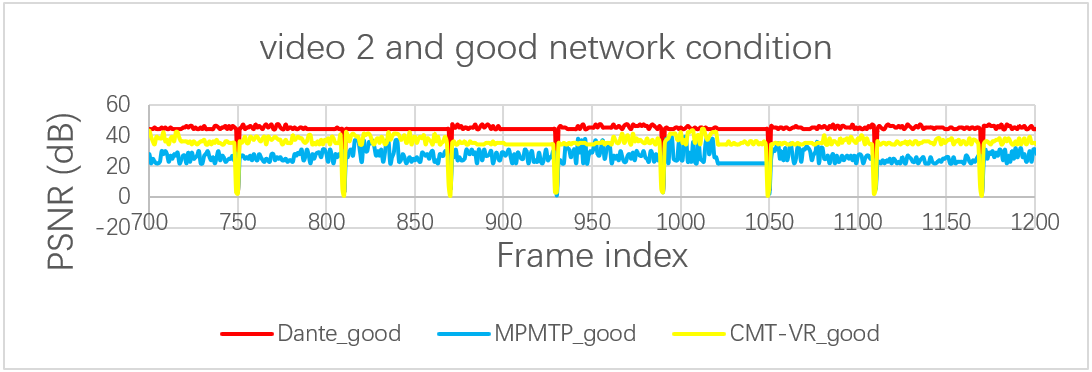
\includegraphics[scale=0.26,angle=0]{paper_figs/evaluation_result/sub/ins_psnr_v2_good.png}}
    % \subfigure[Video Sequence 2]  {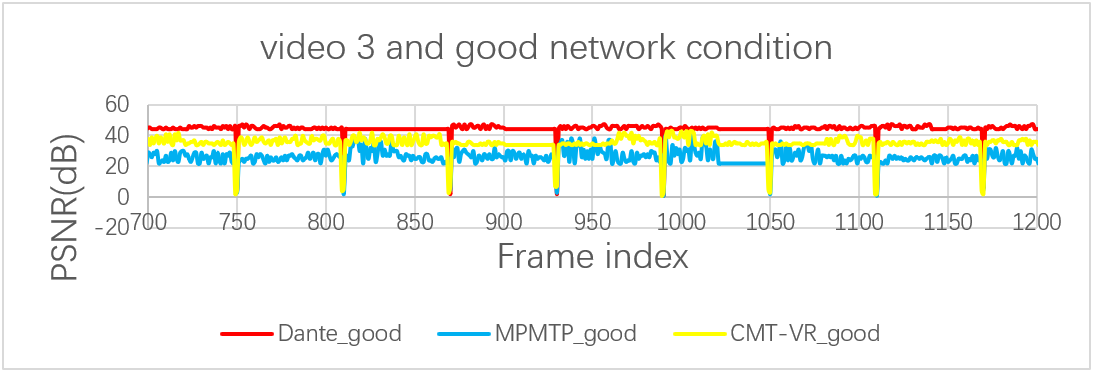
\includegraphics[scale=0.26,angle=0]{paper_figs/evaluation_result/sub/ins_psnr_v3_good.png}}
    \subfigure[Video \#1]  {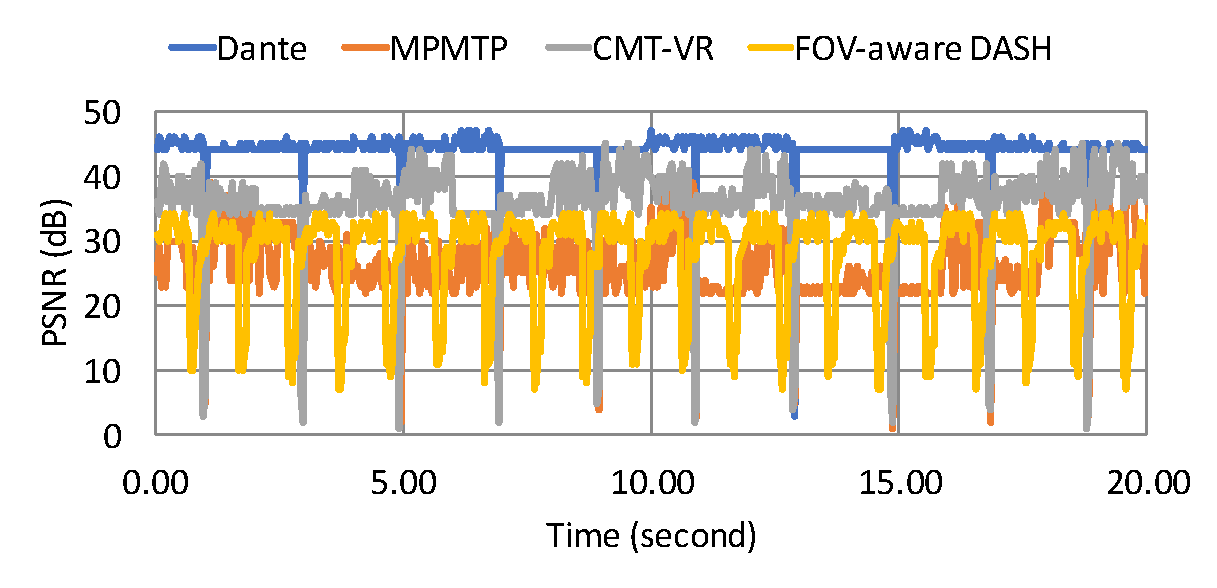
\includegraphics[width=0.4\textwidth]{paper_figs/dante-good-video-1.pdf}}
    % \hspace{-0.3cm}
	\subfigure[Video \#2]  {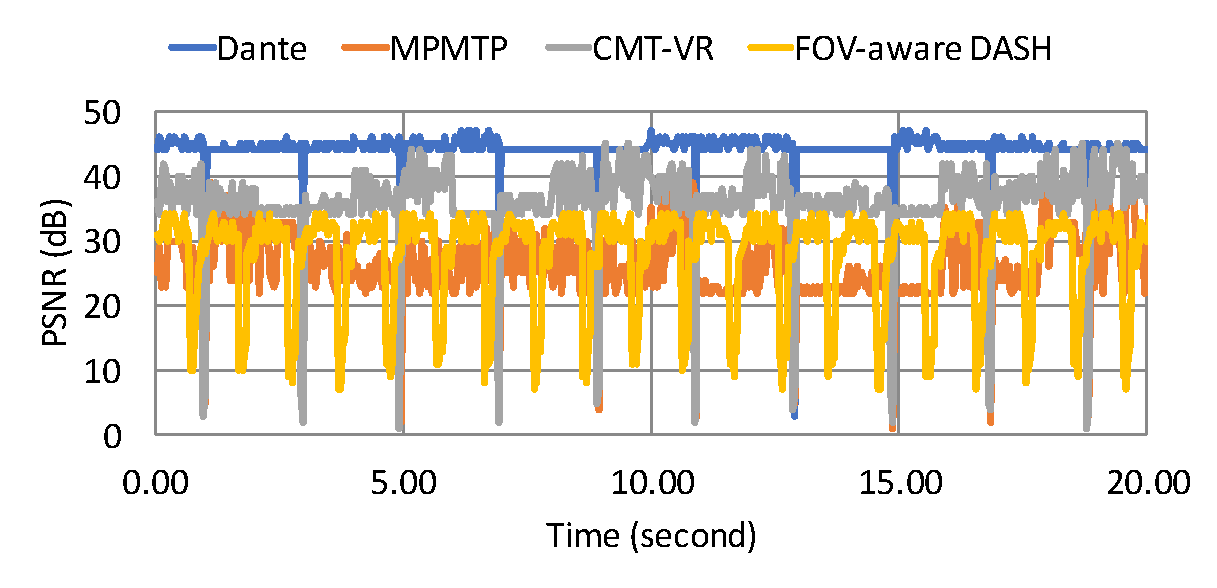
\includegraphics[width=0.4\textwidth]{paper_figs/dante-good-video-2.pdf}}
% 	\vspace{-0.3cm}
	\tightcaption{Dante outperforms three baselines under the relatively good network condition (avg. packet loss rate $=0.5\%$).}
	\vspace{-0.6cm}
	\label{fig:good}
\end{figure*}

%*****Instantaneous PSNR In relatively Good Network Condition*****
\begin{figure*}[!t]
	%\begin{figure*}[t]
	\centering
% 	\subfigure[Video Sequence 1]  {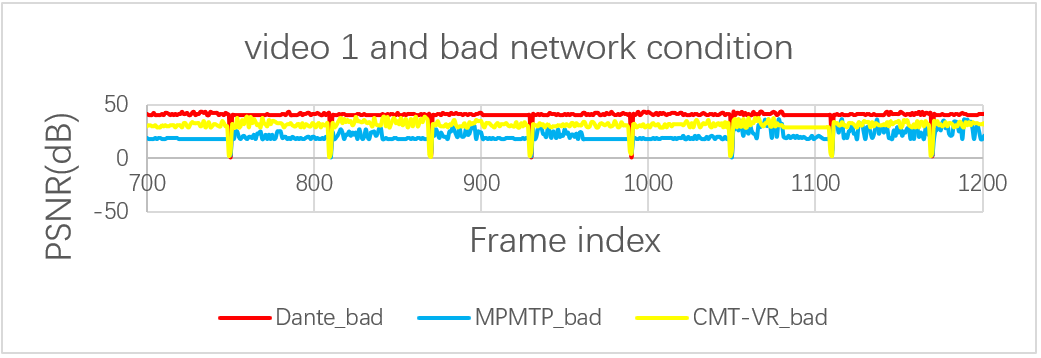
\includegraphics[scale=0.275,angle=0]{paper_figs/evaluation_result/sub/ins_psnr_v1_bad.png}}
% 	\subfigure[Video Sequence 2]  {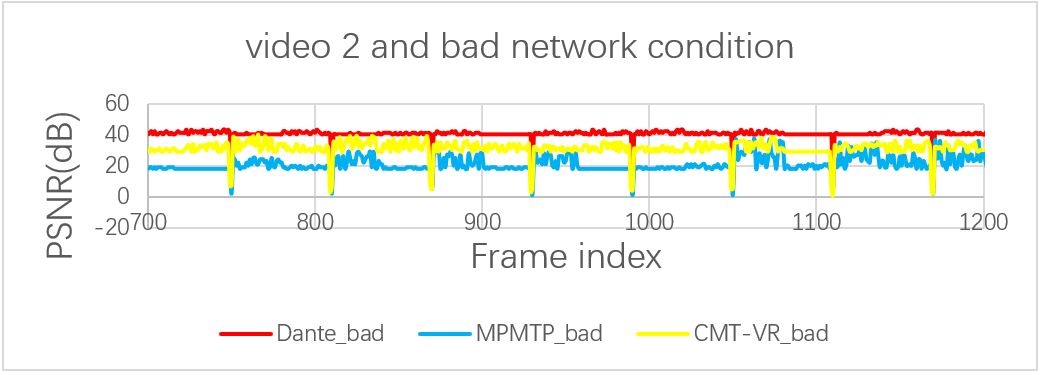
\includegraphics[scale=0.27,angle=0]{paper_figs/evaluation_result/sub/ins_psnr_v2_bad.png}}
    \subfigure[Video \#1]  {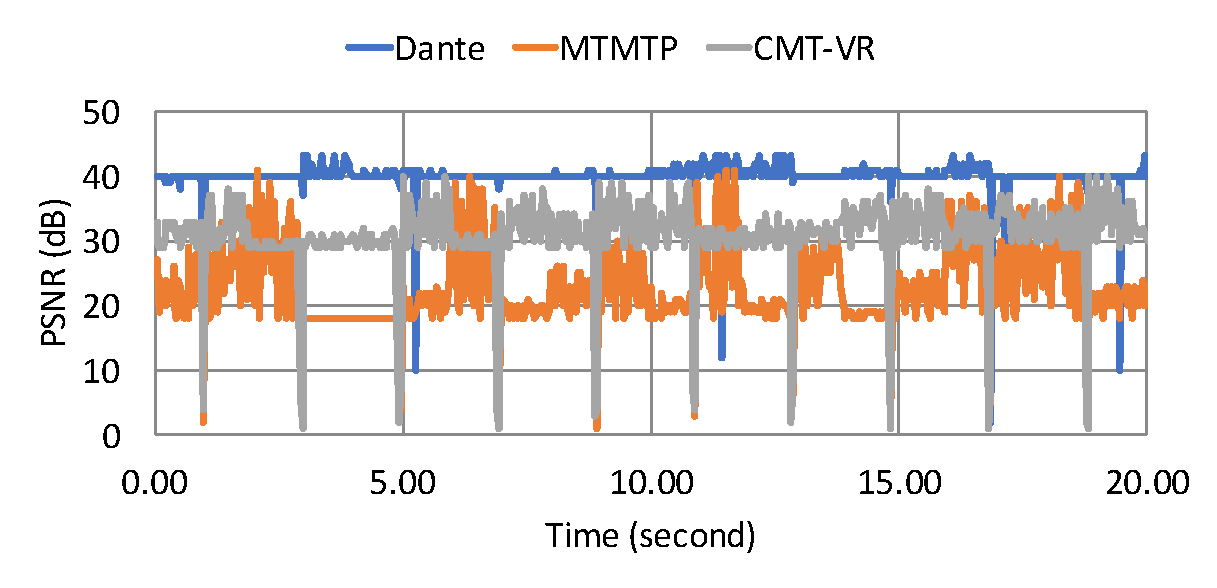
\includegraphics[width=0.4\textwidth]{paper_figs/dante-bad-video-1.pdf}}
    % \hspace{-0.3cm}
	\subfigure[Video \#2]  {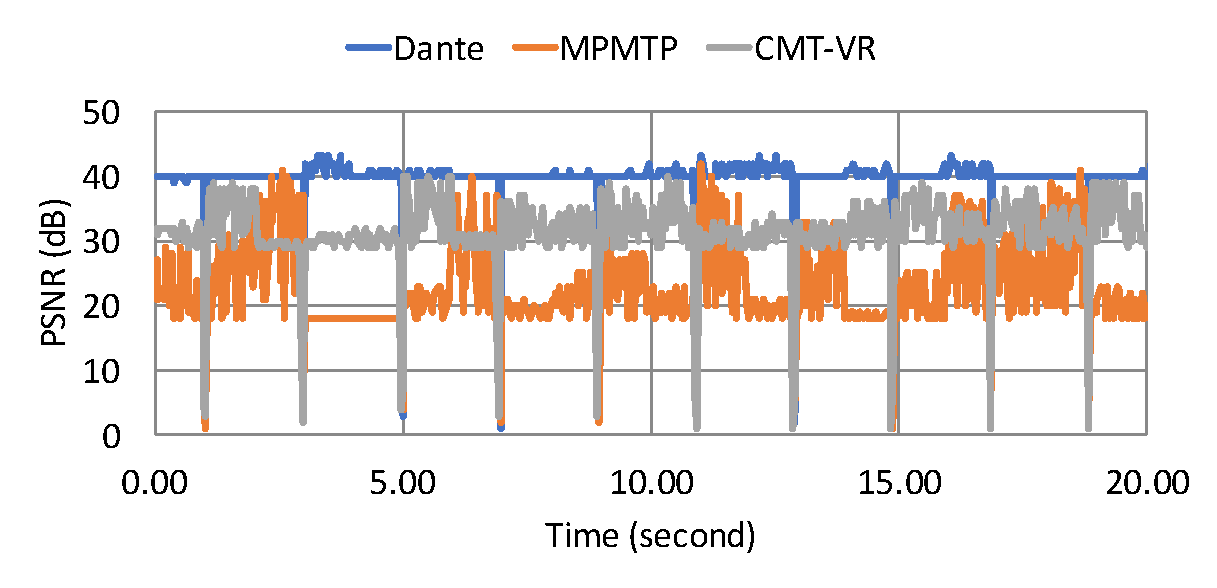
\includegraphics[width=0.4\textwidth]{paper_figs/dante-bad-video-2.pdf}}
% 	\vspace{-0.3cm}
	\tightcaption{Dante outperforms three baselines under the relatively bad network condition (average packet loss rate of 2\%). DASH is not shown here since TCP performs badly under such network condition.}
	\vspace{-0.2cm}
	\label{fig:bad}
\end{figure*}

We use two 360-degree video sequences downloaded from Youtube, 
each of 60 seconds and encoded in H.265 format with a frame rate of 30 frames per second and a GOP size 
of 15 frames. Each frame is split into 72 uniformly 
sized tiles, and we assume users will watch the FOV-region tiles 
(15\% of all tiles) with 60\% probability, cushion-region tiles 
(25\% of all tiles) with 30\% probability, FOV-region tiles (60\% 
of all tiles) with 10\% probability. These settings are aligned 
with prior work (\eg~\cite{360ProbDASH}). Based on this probability 
distribution, we measure the overall quality by the sum 
of PSNR value of each tile weighted by the probability of them 
being watched.

We compare Dante with three baselines:
\begin{packeditemize}

\item {\em FOV-aware DASH}~\cite{Omnidirectional_Video_over_HTTP} 
is built on HTTP/TCP and uses an FOV-aware tile-based streaming 
scheme to reduce bandwidth consumption.

\item {\em MPMTP}~\cite{MPMTP} uses the FEC to recover the data 
without any retransmission. It treats all frames 
separately and thus ignores the interdependency between frames. 

\item {\em CMT-VR}~\cite{CMT-VR} uses quality-driven FEC 
redundancy allocation to minimize the distortion of each GOP and 
Raptor code to avoid retransmission. Unlike MPMTP, it considers 
inter-frame dependency. Both CMT-VR and MPMTP are not FOV-aware. 

\end{packeditemize}




\tightsubsection{Preliminary results}



Then, Figure \ref{fig:good} and Figure \ref{fig:bad} compare instantaneous PSNR of two video sequences in good network condition and bad network condition, respectively. These result show that Dante achieves 20\% to 30\% 360-degree video PSNR performance gain, compared to MPMTP and CMT-VR and 40\% PSNR performance gain, compared to FOV-aware DASH. DASH performs worst since it's underlying TCP protocol achieves poor throughput in high lossy networks. 
The reason why MPMTP also performs badly among these protocols is that, despite maximizing the throughput without any retransmission, it doesn't make extra effort to guarantee the reliability of I frames. So, once I frames can not be recovered from burst packet loss, the GOP of video even can not be normally decoded by video codec and thus resulting in poor performance. Meanwhile, CMT-VR performs better than MPMTP, mainly due to its consideration of frame priority. However, unfortunately, it's non-FOV-aware reliability scheme makes itself waste too much bandwidth on trivial data. Dante takes into account not only traditional video features, like frame priority, but FOV, meanwhile. Benefiting from the hierarchical protection spatially and temporally, Dante achieves desirable upgrade in instantaneous PSNR. Meanwhile, we find, compared to TCP without FEC, the average CPU time of Dante's cients, considering the average CPU time of socket, FEC decoding, video codec as well as rendering, increase from 113\% to 126\%. The almost 11.5 percentage of the extra cpu overhead of FEC can be ignored considering the performance gain Dante achieves.    

\tightsection{Discussion}

\vspace{0.1cm}
\noindent{\bf Why specialized protocols?}
Most solutions of 360-degree video streaming today are built on 
existing HTTP-based protocols designed for traditional 
videos, such as video-on-demand content, 
which are arguably less demanding than immersive 360-degree 
videos in both throughput and delay. While this is not 
without reason (\eg to be compatible with HTTP and reuse CDN servers 
make perfect sense economically), we also see reasons 
to think otherwise. One argument of our work is that specialized 
protocols (FOV-based FEC coding over UDP) can achieve 
significantly better quality. Moreover, Dante is compatible with 
classic streaming stacks like RTP ~\cite{rfc5109}, which have been 
deployed in many legacy services. We leave the question of
deployability of a new specialized video protocol to
future investigation.

\vspace{0.1cm}
\noindent{\bf Relationship to bitrate adaptation:}
Beside deployability, another concern of Dante is how it should 
interact with application-layer bitrate adaptation. On one hand, 
they are functionally complementary. Dante should treat tiles  
encoded with application-specified bitrates as individual files, 
and select FEC redundancy independently to the bitrate of each 
tile. On the other hand, they do affect the performance of each 
other. For instance, if FOV prediction is inaccurate, setting FEC 
redundancy intelligently will not be very helpful, because we 
will probably optimize the video quality of an area not 
eventually viewed. Although the current design of Dante in theory 
is able to work with arbitrary FOV prediction (\ie one can set 
any values for $\gamma_{i,j}$ in Equation~\ref{eq:obj}), it is 
unclear how much FOV prediction accuracy is necessary for FEC 
redundancy adaptation to be useful.

\vspace{-0.2cm}
\tightsection{Conclusion}
This paper proposes Dante, an FOV-aware UDP-based streaming 
protocol for 360-degree videos which leverages the hierarchical 
spatial structure of FOVs. We present adaptive 
FEC coding strategy to prioritize areas that the viewer
is likely to watch. The preliminary results show that Dante achieves
better 360-degree video quality than non FOV-aware UDP-based 
baselines and state-of-the-arts TCP-based baseline.
% protection to counter limited bandwidth and error-prone problems in wireless networks. Experiments demonstrate Dante achieves desirable gains on 360-degree video QoE against reference schemes.  


\vspace{-0.4cm}
\section*{ACKNOWLEDGEMENT}
We would like to thank the anonymous APNet reviewers and our shepherd, Junchen Jiang for their helpful comments.
The work was supported by the National Key Basic Research Program of China (973 program) under Grant 2014CB347800, National Key Research and Development Program of China under Grant 2016YFB1000200 and the National Natural Science Foundation of China under Grant No. 61522205, No. 61772305, No. 61432002. Dan Li is the corresponding author of this paper.

\bibliographystyle{abbrv}
\begin{small}
	\bibliography{apnet18}
\end{small}
\label{last-page}

\end{document}






\begin{figure}[ht]
	\centering
	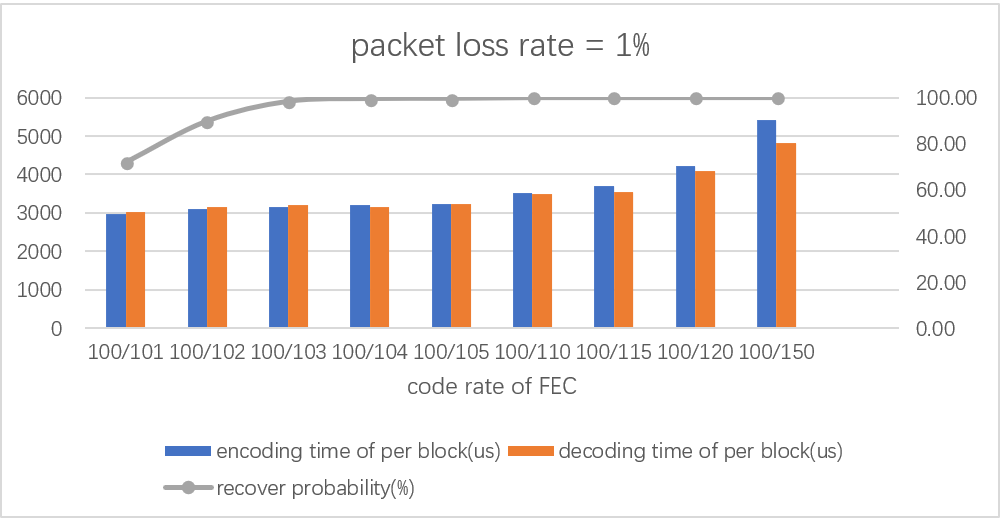
\includegraphics[scale=0.2]{paper_figs/RS_tradeoff.png}
	\caption{Tradeoff between recoverability and goodput}
	\label{paper_figs:pathdemo}
\end{figure}	 

\begin{figure}[ht]
	\centering
	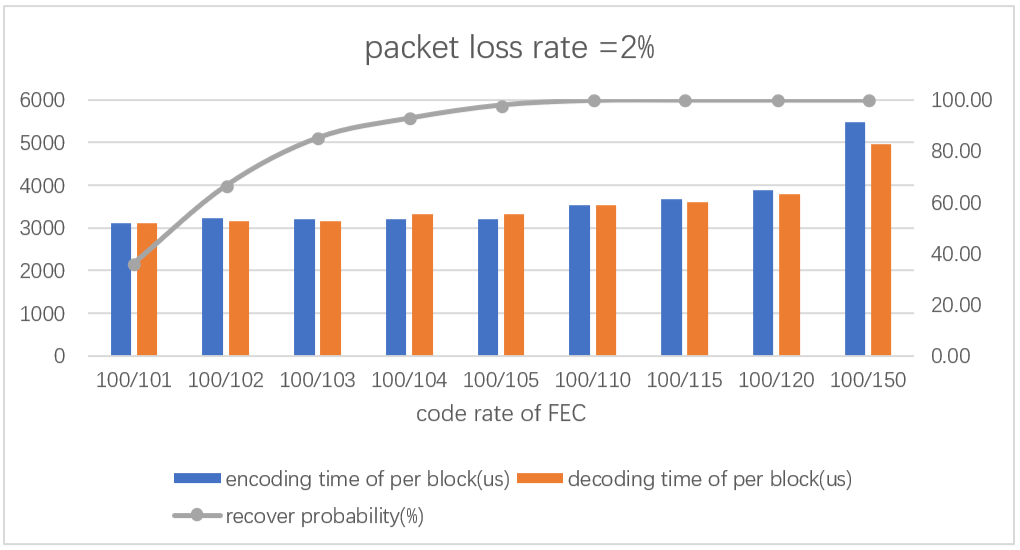
\includegraphics[scale=0.2]{paper_figs/RS_tradeoff_a.png}
	\caption{Tradeoff between recoverability and goodput}
	\label{paper_figs:pathdemo}
\end{figure}	




\begin{table*}
	\centering 
	\scriptsize
	\begin{tabular}{||p{1.35cm}<{\centering}||p{1.5cm}<{\centering}||p{1.7cm}<{\centering}
			||p{1.65cm}<{\centering} ||p{0.85cm}<{\centering} ||p{2.65cm}<{\centering}
			||p{2.0cm}<{\centering} || p{0.85cm}<{\centering} || p{0.85cm}<{\centering}||}
		\hline
		\rowcolor[gray]{0.9}
		\hline
		Solution & protocol layer   & video distortion model & data recovery& adaptive FEC & FEC parameter decision& data
		allocation&video-awareness& FOV-awareness\\
		\hline
		\hline
		MPLOT\cite{MPLOT} & transport layer & $\times$ & RS codes \& retransmissions & \checkmark
		& balance between goodput and recovery probability & packet generation's order & $\times$ & $\times$ \\
		\hline
		FMTCP\cite{FMTCP}    & transport layer  & $\times$ &Raptor codes \& retransmissions &
		\checkmark & balance between goodput and recovery probability & packet
		delivery time minimization & $\times$ & $\times$  \\
		\hline
		MPMTP\cite{MPMTP}  & application layer & $\times$ &Raptor codes & \checkmark & goodput maximization & block arrival time
		minimization & $\times$ & $\times$  \\
		\hline
		CMT-VR\cite{CMT-VR}   & transport layer & inflexible model & Raptor codes \&
		retransmissions & \checkmark & utility maximization& utility maximization &
		\checkmark & $\times$ \\
		\hline
		Dante    &application layer & proposed
		flexible model & RS code & \checkmark & hierarchical
		protection and distortion minimization & hierarchical protection & \checkmark & \checkmark \\
		\hline
	\end{tabular}
	\caption{MAIN DIFFERENCE OF THIS WORK WITH THE EXISTING WORKS}
	\label{}
\end{table*}
